\documentclass[12pt,oneside,final]{siuethesis}
\usepackage{microtype} % (optional) for more beautiful typesetting
\usepackage{graphicx} 
\usepackage{hyperref} %makes links clickable
\hypersetup{colorlinks,citecolor=black,filecolor=black,linkcolor=blue,urlcolor=black} %good for electronic copy
\hypersetup{colorlinks,citecolor=black,filecolor=black,linkcolor=black,urlcolor=black}%required for paper graduate school copy
%\usepackage[alphabetic]{amsrefs} %required if using amsrefs, comment out if using bibtex
\usepackage{fixltx2e}
\usepackage{amsmath}
\usepackage{epsf}
%\usepackage{float}
\usepackage{caption}
\usepackage{subfig}
%\usepackage{subcaption}
\usepackage{listings}
\usepackage{rotating}
\usepackage{tabularx}

\usepackage{multirow}

%% controls numbering of theorems
%% this can be configured to your advisor's taste
\newtheorem{theorem}{Theorem}[chapter] %theorem number resets each chapter
\newtheorem{conclusion}[theorem]{Conclusion}
\newtheorem{condition}[theorem]{Condition}
%% conjectures, corollary, defn, etc. numbered sequentially from beginning of chapters
\newtheorem{conjecture}[theorem]{Conjecture} 
\newtheorem{corollary}[theorem]{Corollary}
\newtheorem{example}[theorem]{Example} 
\newtheorem{lemma}[theorem]{Lemma}
\newtheorem{proposition}[theorem]{Proposition}
\newtheorem{solution}[theorem]{Solution}
\theoremstyle{definition}
\newtheorem{definition}[theorem]{Definition}


\author{Monjur Ellahi Rafi}
\title{A Custom IC for Silicon Strip Detectors \protect\\
Employing the Use of Dual Shapers}

%%\advisor{John Q.\ Faculty} %% or 
\advisor{Dr.}{George L. Engel}
\secondreader{Dr.}{Bradley Noble} %% or \secondreader{Dr.}{Karl Gauss}
\thirdreader{Dr.}{Timothy York}
%\fourthreader{Karl Gauss, Sr.}
%\fifthreader{Karl Gauss, Sr.}
%\secondadvisor{Karl Gauss} %if you haves two advisors (rare) then use this line also and pass the option `twoadvisors' to the class
%\abstracttext{Chairperson: The Honorable Jill Smith} %optional -- you can use this to override the text on the abstract page; the grad school default is built-in
\submitdate{August, 2018} %date the month/year submitted to grad school, use a comma between
\copyrightyear{2016} %optional, but required if copyrighted

%% all of these are optional; defaults are shown
\major{Electrical Engineering} 
\degree{Master of Science} %can be used to specify M.A., etc.
\highestdegree{Bachelor of Science} %used if the author already has another graduate degree
\department{Electrical and Computer Engineering} 
%\departmentname{Department}
%\refname{REFERENCES} 

%\captionsetup{width=0.7\textwidth}

\begin{document}
\maketitle 

\frontmatter %signals single spacing/roman numeral pagination

\copyrightpage %optional

%%% abstracts are optional
\begin{abstract}

Robotics is a fast growing field with a wide variety of applications. With the advent of new, compact, and cheap computing solutions, the user community and hobbyist markets are expanding rapidly. Robotic competitions are also becoming extremely popular among students in engineering programs across the country. Achieving reliable, accurate movement is one of the most challenging aspects of any robot, and most of the current platforms out on the market do not provide the level of performance or the necessary degree of flexibility that autonomous robot competitions at the university level demand. 

Using a popular yet inexpensive single-board computer \emph{i.e.} the Texas Instruments' BeagleBone Black, a custom circuit board (the SIUE Robot Cape), and \emph{Makeblock}\textsuperscript{\textregistered} (mechanical parts), a small, easy-to-use, yet powerful robotics platform has been developed. The platform supports either four DC motors with quadrature wheel encoders or two stepper motors running open-loop. The ability to independently control four DC motors with encoder feedback affords the user the option of employing four omni-directional wheels in the design of the robot.

In addition to providing reliable movement, the SIUE (Southern Illinois University Edwardsville) Robot Cape, described herein, supports two I2C (Inter-Integrated Circuit) buses, a RTC (Real-Time Clock), a 16-channel servo motor controller, and a 9 DOF (Degree of Freedom) accelerometer. The system can be powered from standard RC car NiMH batteries.  The overall system strikes the right balance between flexibility and ease-of-use. In the pursuit of this end, a graphical user interface was developed to allow users to quickly configure the system.

A very simple demonstration robot, using a pair of DC motors with optical wheel encoders, is described in the thesis. A cascaded PID (Proportional, Integral, Derivative) controller is employed.  A PID loop (slave) for each motor controls wheel velocity while a third (master) loop drives the difference in wheel velocities to zero. The output of the master loop adjusts (differentially) the velocity setpoints of the left and right motors. When tested, the robot performed well on tests used to assess robot movement employing odometry.

\end{abstract}

\begin{acknowledgements}


First, I want to deeply thank my committee chair, Dr. George Enge,l who has been a wonderful and supportive teacher and without whose help and support this thesis could not be possible. 

I would also like to thank my other committee members, Dr. Brad Noble and Dr. Timothy York, since they have been indispensable to my studies. I also want to extend my thanks to other professors who have helped me achieve my goals:  Dr. Andy Lozowski, Mr. Steve Muren, Dr. Ying Shang, Dr. Scott Smith, and Dr. Scott Umbaugh.

I am forever indebted to my parents, Terry and Sara Faber, and my sister, Libby Faber, for their unconditional love and support throughout the years.  They has given me strength through the good and bad times. Thank you. Without you, this thesis would not have been possible.

I also thank all of my friends for their support and camaraderie throughout this crazy journey. I especially want to thank Christian Cool, Luke Hunt, Tyler Mustard, and Mark Ostroot who have helped me in their own ways. I am only as tall as the shoulders I stand on. You all have my deepest gratitude.

\end{acknowledgements}

\tableofcontents

\cleardoublepage %cause correct numbering of list of figures

\listoffigures %print list of figures page

\cleardoublepage

\listoftables

\mainmatter %signals single spacing/arabic numeral paginations


\chapter{INTRODUCTION}  %% chapter titles must be typed in all caps to conform with regulations


\section{Growing World-Wide Interest in Robotics}

As computing power increases and form factor decreases, increased emphasis has been placed on robotics as a means of problem solving.  Robots can be used to automate and simplify processes that would otherwise require large amounts of manpower, or they can make a work environment safer by taking the human element out of the equation. The scale of robotics applications ranges from industrial assembly, using large-scale control systems and powerful motors, to hobbyist, using small low-powered computing systems and simple components.

Hobbyist robotics is a growing field accompanied by an ever increasing number of competitions both for academic and recreational purposes and has spurred a thriving industry to support these endeavors.  Moreover, robotic competitions are becoming extremely popular among students in engineering programs across the country, and most electrical and computer engineering programs in this country offer courses in robotics.  Class projects in robotic courses often involve competition.

Frequently, teams will buy pre-made boards or kits that provide certain specialized functionality such as sensors for environmental feedback or movement via servos or motors. A combination of these are typically used to complete objectives in a course.  During competition, a robot is generally required to \emph{move} through a course and complete a series of specified tasks along the way. There is a large variety of styles and mechanisms for achieving accurate and reliable movement but probably the most popular and easiest method is to use a wheeled-type robot utilizing a motor controller of some sort.

Electrical and Computer Engineering students at SIUE (Southern Illinois University Edwardsville) have, for the last 20 years or so, participated in autonomous robotics competitions sponsored by Region 5 of the IEEE (Institute of Electrical and Electronic Engineers) professional society. Students have generally built a robot from scratch for each competition using available hobbyist parts or have purchased robot kits. 
 
\section{Motivation for Thesis Work} 

The author's personal experiences while working on a a robot, pictured in Figure~\ref{fig:FaberRobot},for the aforementioned IEEE competition was the motivation for the work described in this thesis.  The author was disappointed by the robot's performance in competition. A large amount of time and energy went into trying to deal with simple mechanical issues.  Reliable, accurate robot movement was also a major problem. 

\begin{figure}[htbp!]
\centering
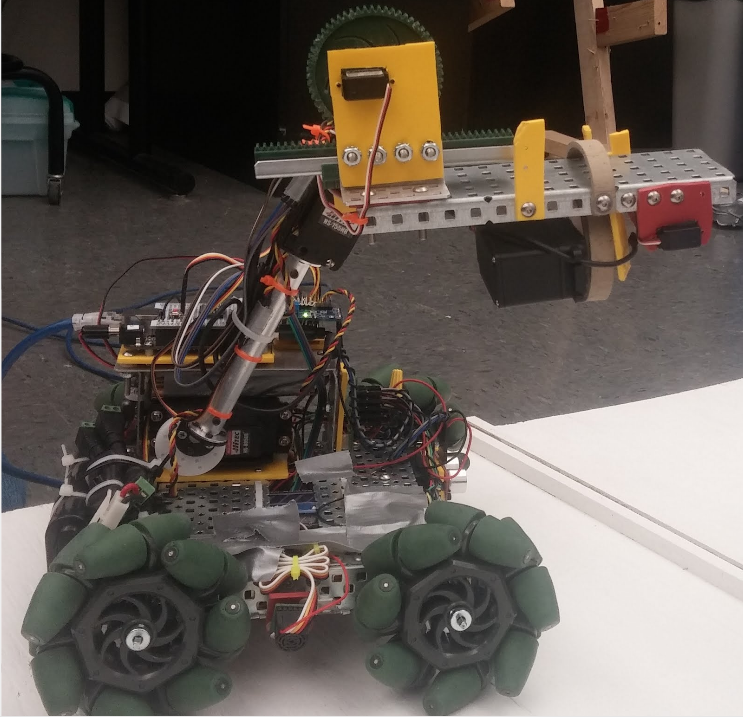
\includegraphics[scale=.6,keepaspectratio=true]{./images/FaberRobot.png} 
\caption{Authors's Robot for IEEE Competition}
\label{fig:FaberRobot}
\end{figure}

The author reached the following conclusions: (1) complete robotic platforms currently available are not versatile enough to meet the demands of university-level, autonomous robot competitions and (2) successfully completing contest-specific tasks is sufficiently challenging without students needing to worry about reliable robot movement.  After researching available options, it became clear that recent advances in so-called single-board computers (SBC) offer an opportunity to improve the chances of future SIUE robotic teams performing well in autonomous mobile robot competitions. 

Past experience suggests that the overall robotics platform must contain the following elements if a team is to be successful in an autonomous mobile robot competition:

\begin{itemize}
\item 
mechanical components to construct a mechanically-sound robot,
\item
a high-performance, small form factor computer platform that can be used for high-level decision making,
\item
an intelligent, flexible, dedicated motor controller highly integrated with the high-level compute platform, 
\item
a method to quickly and easily integrate peripheral devices into the robotic system, and
\item
a quick and convenient way to change system parameters, thus promoting experimentation.
\end{itemize}

\noindent
With the requirements above as a guide, the following objectives for the thesis work became clear.
\begin{enumerate}
\item
Identify a maker of mechanical robot parts which are inexpensive, easy-to-use, and flexible. Students should \textbf{not} have to machine their own parts nor should they be constrained to use a prescribed robotics kit.
\item
Identify a SBC that would be able to handle the requirements of both movement and higher level decision making.
\item
Create a custom motor controller board capable of handling all motor types which could be highly integrated with the processor tasked with higher level decision making. The board should also contain key peripherals and the ability for the user to quickly and easily add additional peripherals.
\item
Create a graphical user interface (GUI) that would allow students to quickly configure the key parameters of the robotic system.
\end{enumerate}

\noindent
In the following section, we briefly describe the various types of motors generally encountered in robotic applications.

\section{Types of Motors Used in Mobile Robotics}

% RobotShop website should be cited

Traditionally, three types of motors are used in robotics: DC, stepper, and servo. In a continuous DC motor, application of power causes the shaft to rotate continually. The shaft stops only when the power is removed, or if the motor is stalled because it can no longer drive the load attached to it.  In a stepping motor, applying power causes the shaft to rotate a few degrees, then stop. Continuous rotation of the shaft requires that the power be pulsed to the motor.  A special case of continuous DC motors is the servo motor, which in typical cases combines a continuous DC motor with a “feedback loop” to ensure accurate positioning. A summary of the advantages and disadvantages of each motor type is presented in Table~\ref{Tab:Motor_Types}.  

As is made clear by looking at the table, the three motor types have advantages and disadvantages. The task is for the user to choose the right motor for the application. It is important that all three types of motors be supported. For example, while locomotion is perhaps best handled by a DC or stepper motor, opening and closing a gripper for grabbing objects is best accomplished with a servo motor. All three motors need to be "controlled" and in the following section we review motor controllers.

\begin{table}[htbp!]
\begin{center}
\begin{tabular}{|p{0.75in}|p{2.5in}|p{2.5in}|}
\hline
Type & 
Advantages & 
Disadvantages\\
\hline
DC & 
Wide selection available. Many come with gear boxes so high torque, low-velocity operation is possible. & 
Poor standards in sizing and mounting arrangements.\\
\hline
Stepper & 
Does not require gear reduction to power at low speeds. Dynamic braking achieved by leaving coils of stepper motor energized (motor will not turn, but will lock in place).& 
Poor performance under varying loads. Not great for robot locomotion over uneven surfaces. Consumes high current.\\
\hline
Servo & 
Inexpensive. Can be used for precise angular control, or for continuous rotation. Available in several standard sizes, with standard mounting holes. & 
Practical weight limit for powering a robot is about 10 pounds.\\
\hline
\end{tabular}
\caption{Comparison of Motor Types Used in Robotics.}
\label{Tab:Motor_Types}
\end{center}
\end{table}


\section{Motor Controllers} 

There are many motor controllers on the market which range from simple H-Bridge drivers to full-blown computing boards that implement some type of control using feedback from the motor. One controller on the market that a past SIUE robotics team used was called the \emph{SSC-32}, manufactured by \emph{Lynxmotion}. This board used an ATMEGA168A to provide PWM (Pulse-Width-Modulation) control to servo motors connected to the board powered with an external power supply.

Commands to this board were received via a serial interface that could be either RS-232 or UART (Universal Asynchronous Receiver Transmitter) compliant based on jumper configuration. One major problem with this board was the lack of feedback. It only supported continuous rotation servos. These motors are adequate for very small, lightweight robots but can produce very little torque, thus rendering them useless for use with larger, heavier robots.
	
Another controller board used by a past team was the \emph{Serializer} manufactured by \emph{Robotics Connections}. This product was later produced by \emph{cmRobot} under the name \emph{Element} but it is now obsolete.  The \emph{Serializer} was sold as a complete robotics board with on-board CPU, memory, I2C (Inter-Integrated Circuit) connections, servo ports, analog inputs, and dual motor H-bridges with encoder input. The board was designed so that users could start working on projects quickly, giving the user immediate access to the functionality of the board. 

However, the board existed as a closed system and could only accept a small, fixed set of commands via a serial port. The closed system aspect of the \emph{Serializer} was a major problem for robotic teams. The lack of flexibility frustrated students. When using I2C functions one could use the libraries provided for certain parts but if an unsupported device was used, a read had to be done for each individual byte. The PID functionality of the board was nice but it was difficult to tune the system for different motors and platforms because it had to be done on every boot of the system. 

Furthermore, the serial port, while being ubiquitous in most applications, caused problems for past teams. When using the serial port in a C programming environment, which is typical of most smaller embedded computer systems, data comes back in a character array format followed by a null terminator. If data was being read from the system, the user would have to take the time to first parse the array and then make the conversion from characters to numbers that could be used by the system. This becomes a very tedious process for programmers. Other issues with the board would be that serial communication would often disconnect due to poor connections, causing a massive headache for teams. The board was usable, but it was not as flexible as one would like.  

In an attempt to address some of the issues described above, a custom board was created, in the same spirit as that of the \emph{Serializer}, by the author's thesis advisor. This board (see Figure~\ref{fig:PSoC_board}) used a PSoC 1 microprocessor made by Cypress Semiconductor along with Texas Instrument H-Bridges to control a pair of DC motors with feedback from wheel encoders. The board also supported two servo motors and a single I2C bus. It did \textbf{not} support stepper motors. Initially, this PSoC-based board was used for \underline{both} motor control and high level decision making, but it soon became clear that it lacked sufficient computing power to perform both tasks.

\begin{figure}[htbp!]
\centering
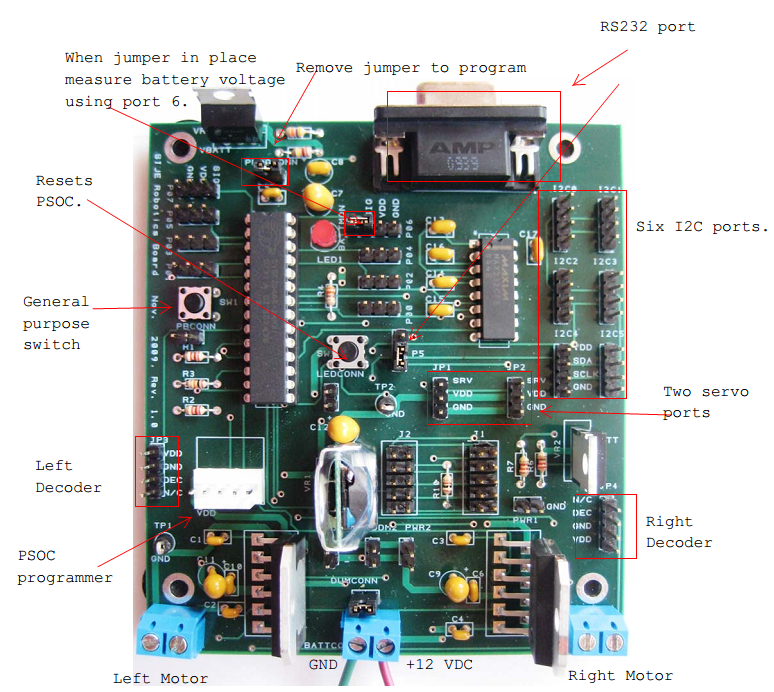
\includegraphics[scale=.75,keepaspectratio=true]{./images/PSoC_board.png}
\caption{SIUE Motor Controller Board Using Cypress PSoC}
\label{fig:PSoC_board}
\end{figure}


The PSoC 1 is a microprocessor that is highly versatile with programmable digital modules to implement a wide variety of counters, communication protocols and analog devices all controlled by a signal CPU. The PSoC served as the heart of this board, implementing PID functionality for two DC motors with encoder signal feedback for each motor.  Along with the motor controller, this board provided line following capability to allow a robot to follow black lines on white surfaces which could be used to keep the robot on course.  Other functions of the board included servo motor controllers, I2C interfacing, and GPIO (General-Purpose Input/Output) connections. This board solved some of the problems associated with the \emph{Serializer}, but had its own set of issues. 

Again, this board used a serial port to communicate with a host and much like the previous board, communication would sometimes be sporadic on the robot due to the potential for connections to break.  Also, there was a limited amount of information that was transmitted back to the host system, mostly just acknowledgments that the system had completed the process that it was given. In some situations the host system would hang when waiting for an acknowledgement signal because something had either gone wrong on the PSoC board or the acknowledgement had been lost in transmission. When adjusting and tweaking, it is helpful to view values that were read and calculated, but there was no memory dump for the host system. When values needed to be changed, the program for the PSoC needed to be recompiled in the IDE (Integrated Design Environment) that is only available through Microsoft Windows and then programmed through a USB (Universal Serial Bus) programmer. 

This approach did not allow for on-the-fly tweaking of PID (Propotional, Integral, Derivative) parameters which resulted in a slow tuning process for the PID controller. Things like wheel diameter, ticks per rotation, and PID gain all had to be reprogrammed into the PSoC. A more useful approach is \textbf{not} to use serial communication but rather have one system that handles both the high level decision making and handling of the motors and other peripheral devices. As mentioned above, the PSoC lacked sufficient power to handle both tasks. A more powerful system such as a SBC is needed if one system is to handle all of these tasks.


One motor controller board that is designed to use a SBC (Single-Board Computer) is the DMCC (Dual Motor Controller Cape).  It was designed by \emph{Exadler Technologies Inc} for the Texas Instruments' BeagleBone Black and is described in detail in a later section. This board (see Figure~\ref{fig:DMCC} is used to control two motors with H-Bridges that can supply up to 7 Amps at 5 to 28 volts~\cite{DMCC}. 

There is no datasheet available for the board, but there are github repositories. After some exploring of the repositories, it appears that this cape is controlled by a dsPIC33FJ32MC304 by Microchip which is a 16-bit micro-controller with 8 PWM channels and two quadrature encoder interfaces. It appears that the micro-controller is accessed by the BeagleBone Black via I2C communication for setup and control. 

The software is a collection of functions to access the I2C bus and send data to the micro-controller for setup and operation. PID control is implemented on the micro-controller and can be used to control either the velocity or position of the motors. This is again a closed system, similar to the \emph{Serializer}, because the firmware on the micro-controller is pre-loaded and source code is not provided. It is only the DMCC that can truly be considered a direct competitor to the board designed for this thesis.  In the following section, we will review SBCs \emph{i.e} single board computers.\\

\begin{figure}[htbp!]
\centering
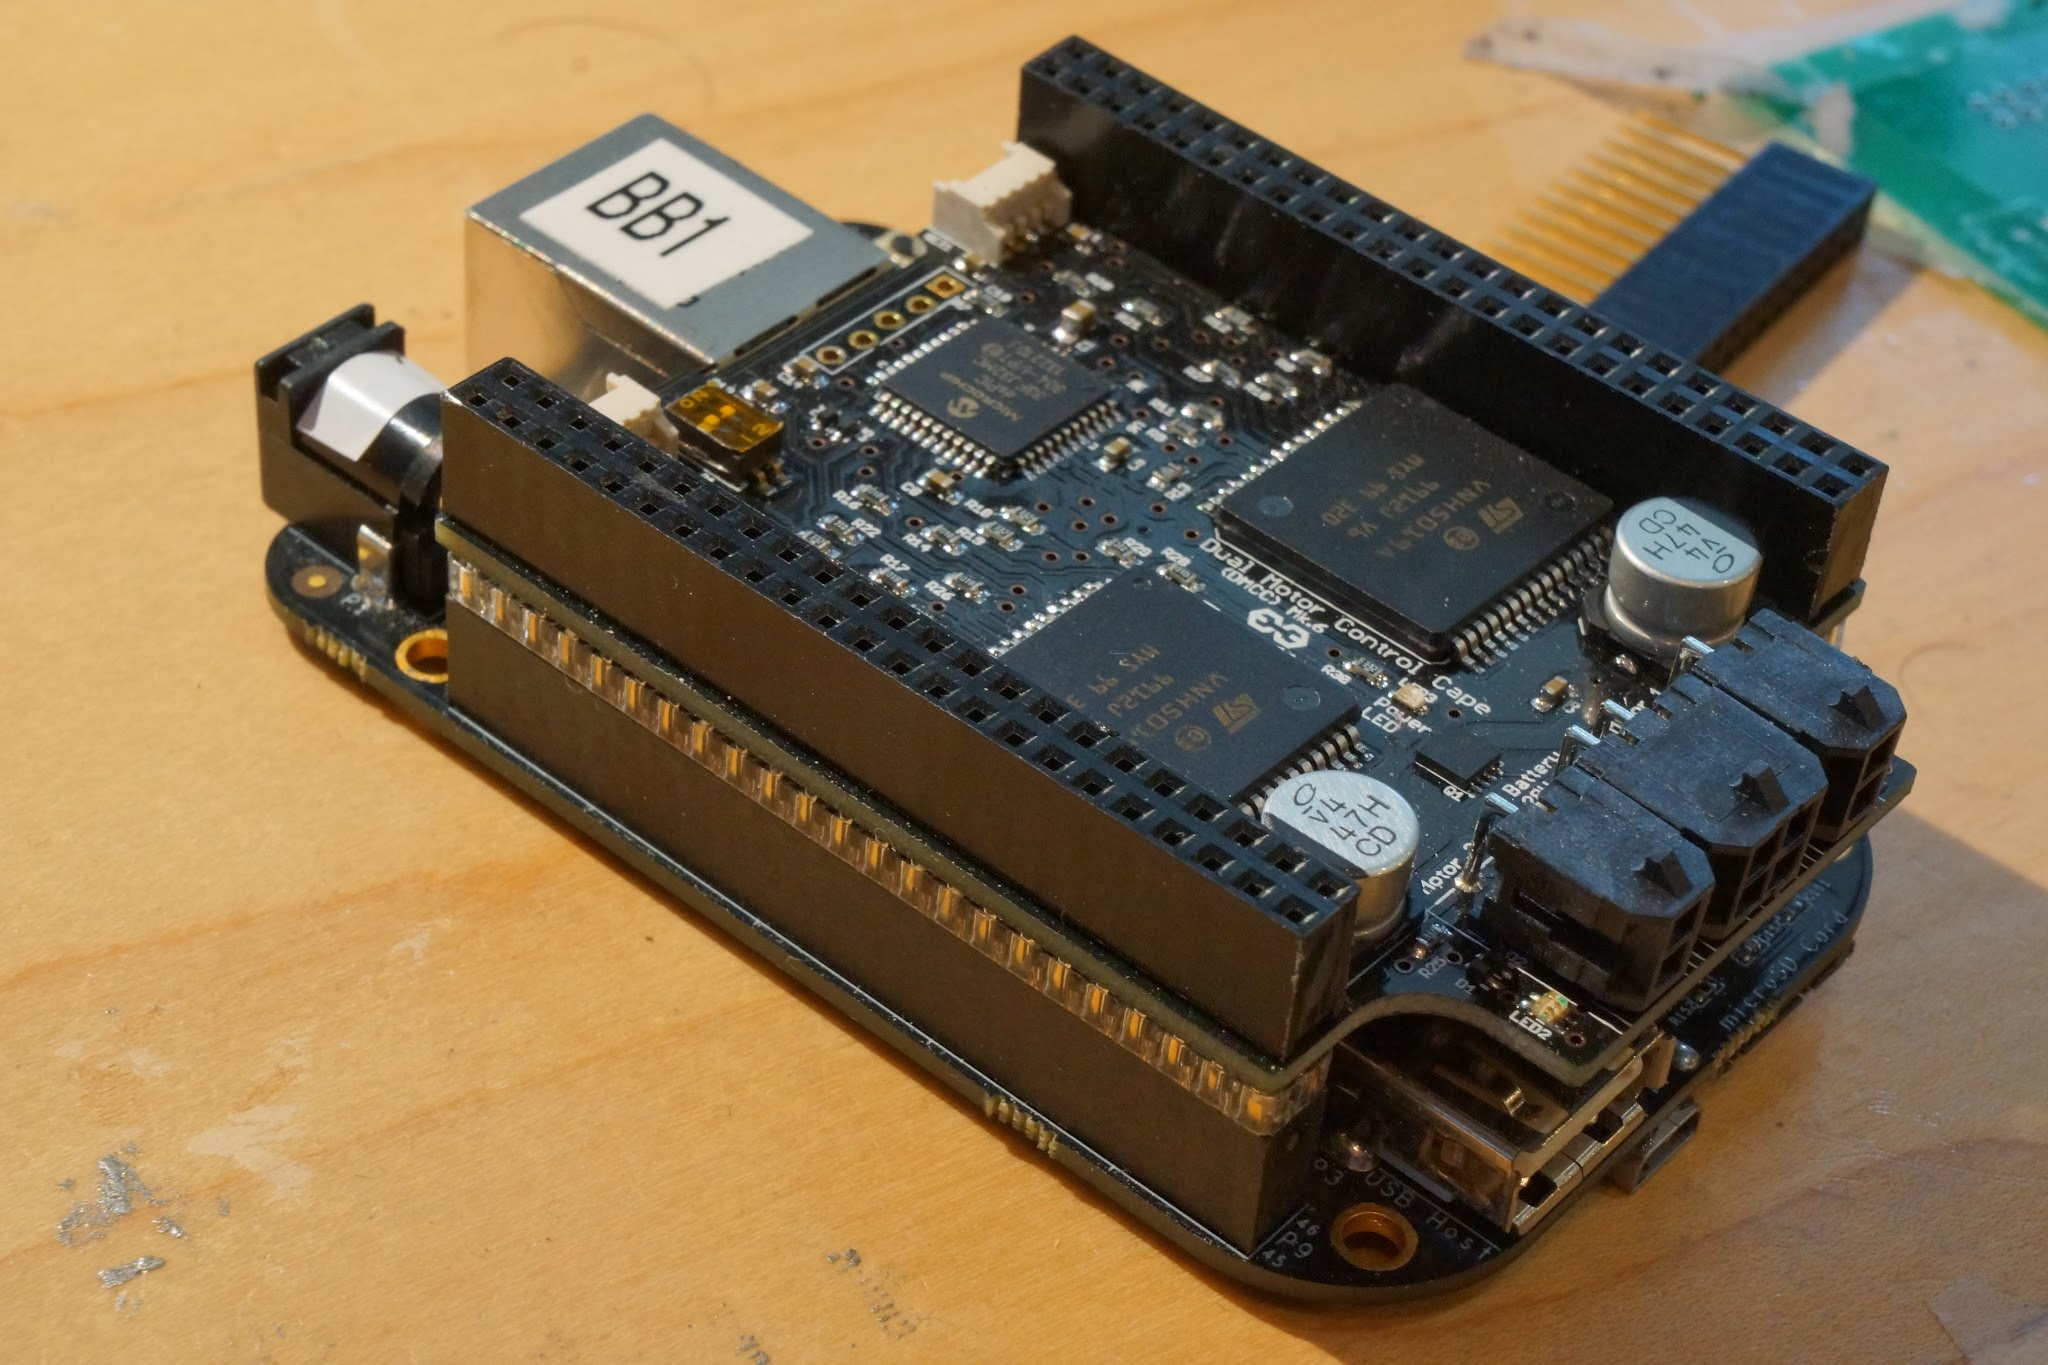
\includegraphics[scale=.15,keepaspectratio=true]{./images/DMCC.jpg}
\caption{Dual Motor Controller Cape (DMCC)}
\label{fig:DMCC}
\end{figure}

\section{Single-Board Computers} 

Single-board computers (SBCs) have been around for quite some time and have recently grown in popularity as integrated circuits decrease in both size and price. One of the most prolific devices currently out on the market is the \emph{Arduino} which is more aptly described as a micro-controller rather than a SBC, but it is often mistaken for one.  While the Arduino is powerful, complete with analog and digital I/O, it has limits when it comes to intense calculations or tasks that are better suited for full-blown computers. 

The Raspberry Pi is one of the most popular SBCs currently out on the market, and it has taken both the hobbyist and teaching communities by storm. The small size of the system along with the low power consumption, which permit it to operate off a USB connection, make it easy to use and accessible to the general public. The system runs a custom version of Debian called Raspbian which is a widely used Linux distribution and comes with the ability to be hooked up to a monitor with keyboard and mouse and used as a full-fledged computer. 
	
The board also has digital I/O pins which can be used to implement a wide variety of protocols such as I2C or UART as well as implementing general digital I/O functions. The combination of a full-blown operating system along with microprocessor functionality makes for a potent combo in a robotics platform. Over the last couple of years, upgraded models have been released. The Raspberry Pi 2 and  Pi 3  have increased performance over the original Pi, and the Pi Zero which is less than half the size of the original Pi. A comparison of the various Raspberry Pi offerings is presented in Figure~\ref{fig:Pi_offer} ~\cite{RPi3}. While these devices are very powerful, especially the recently released Raspberry Pi 3, they are actually better suited for multimedia applications such as console/arcade emulation and media box creation than for mobile robotic applications.

\begin{figure}[htbp!]
\centering
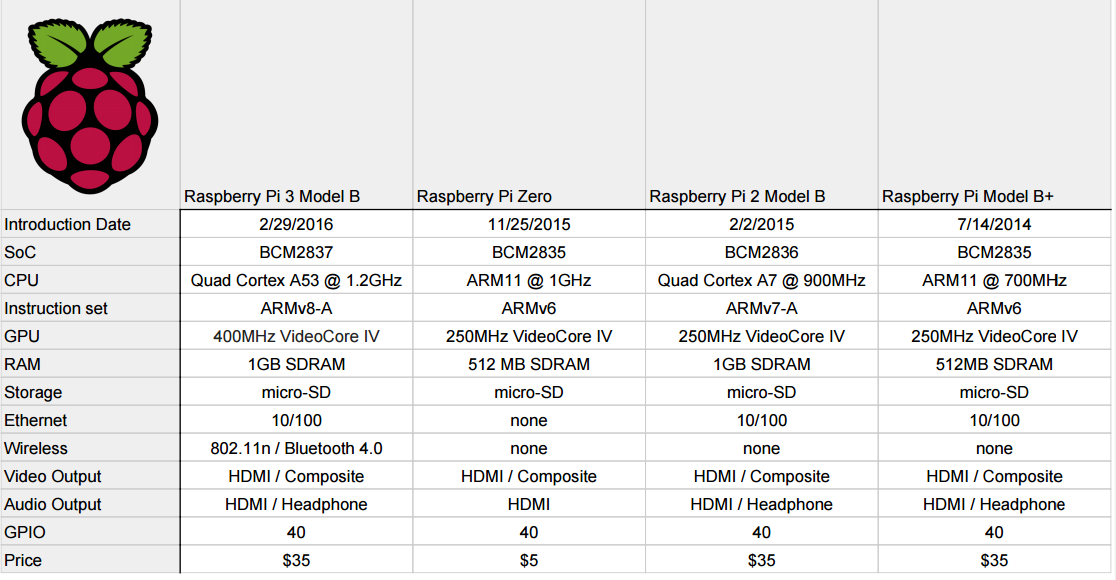
\includegraphics[scale=.4,keepaspectratio=true]{./images/pispecs2.png}
\caption{Raspberry Pi Offerings }
\label{fig:Pi_offer}
\end{figure}


A direct competitor to the Raspberry Pi is the BeagleBone Black which will be described in the following section.  It is the BeagleBone Black that was selected for use in this thesis work. The rationale for this decision will also be presented.

 


\section{Object and Scope of Thesis}

The goal of this thesis is to integrate a single-board computerwith a motor controller/periphearal board to make it easier for future robotics teams and hobbyists to quickly assemble a mobile robot. The hope is that the work presented in the thesis can be used by student groups at SIUE in the future as a solid foundation for the creation of robots which can be competive in  autonomous robotic contests.

In Chapter 1 of this thesis, we have discussed the growing interest in mobile robotics, the various types of motors which are used in robotic applications, and the motivating forces for this work.  We then went on to review motor controller boards and single board computers. We concluded with an overview of the Texas Instruments' BeagleBone Black single board computer which will be used throughout this work.

Chapter 2 presents a detailed decription of the design of a daughter board (known as a "cape") for the Beaglebone Black.  The SIUE Robot Cape described in Chapter 2 supports either four DC motors with quadrature wheel encoders or two stepper motors running open-loop. The ability to independently control four DC motors with encoder feedback affords the user the option to employ four omni-directional wheels in the design of a robot. In addition to providing reliable movement, the SIUE robot cape provides access to two I2C buses, a real-time clock, a 16-channel servo motor controller, and a 9 DOF (Degree of Freedom) accelerometer. 

In Chapter 3 the software developed for the two BeagleBone Black PRUs (Programmable Real-Tine Units) is described.  The chapter starts with a description of the contents of the memory which is shared between the two PRUs and the ARM core. This shared memory provides tight integration between the user code running on the ARM and the motor controller code running on the two PRUs eliminating the need for serial communication between compute platform and motor controller! The chapter goes on to describe the PID algorithms used to ensure high quality movement employing odometry provided by optical wheel encoders. The code developed for each of the two PRUs is decribed in detail.

Chapter 4 presents the development of demonstration robot used to evaluate the quality of movement. The chapter begins with a description of the robot frame using MakeBlock mechanical components. The chapter goes on to describe the routines in a series of libraries which were created to jump start future robotic teams. The chapter continues with a description of the Graphical User Interface (GUI) which was created to allow users to quickly change system parameters. The chapter concludes with a discussion of a demonstration program and present results of tests which were run to quantify the quality of the robot movement. A summary, concluding remarks, and some suggestions for future work are provided in Chapter 5.

\chapter{SYSTEM LEVEL DESIGN}

\section{Hardware Design Objectives}

In this chapter the design of a daughter board that can be plugged into the BeagleBone Black, using the P8 and P9 connectors, is described.  The daughter board provides the necessary hardware to interface and control the motors and other popular peripherals. Daughter boards that give added functionality to the BeagleBone Black are called \emph{capes} which have their own unique overlay to describethe pin multiplexing that is required for the board to connect correctly to the various peripheral devices. 

The cape overlay system has the added benefit of having a plug and play functionality which on boot, if the cape is present in the firmware, can be loaded.  First, the system level design of the board will be presented and then a short discussion of how the overlay system for a cape works is given. We conclude with a discussion of the peripherals available on the cape.

The main goal of the SIUE Robot Cape was to provide the user with motor drivers that are capable of handling modest amounts of power while retaining a small form factor. In addition to motor drivers, appropriate level shifting was required by the motor encoder signals to ensure that only a 3.3 volt signal would be presented to the BeagleBone Black input pins. Any voltage higher than 3.3 volts on any digital pin pose a hazard to the Black. Additional peripheral devices were added to the board if they were deemed either extremely useful for robot designers and/or provided infrastructure for commonly used communication protocols. 

Physically, we desired a two-layer board with one layer being a ground pour. We used surface mount components on the top layer which helped save on space because of their typical small form factor compared to through hole parts. Finally, the board was designed in a manner so as to isolate the digital and high power circuits from one another as much as possible by having the high powered components located on an outcropping away from the digital electronics so that there would be a reduced chance of crosstalk which might in turn cause unexpected problems.


\section{System Overview}

The final version of the SIUE robot cape is pictured in Figure~\ref{fig:board_diagram}. Onboard chips include H-Bridges for the motor driving circuits, buffers for the inputs and outputs of the PRU pins, a quad XOR gate for use with the quadrature encoder input signals, an I2C level shifter, a pair of LEDs, two momentary switches, and an EEPROM (Electrically Erasable Programmable Read Only Memory) for board loading.  In addition there are two additional break out boards, an accelerometer and a real time clock, along with an additional EEPROM that can be accessed through the I2C bus and used by the ARM or PRUs if desired. There is also a place to add a 16-Channel servo driver board.  After a discussion of board setup and configuration, the peripherals available on the board will be described in more detail. 

%TODO need to redo this at some point get a better image
%
%\begin{figure}[htbp!]
% \centering
% 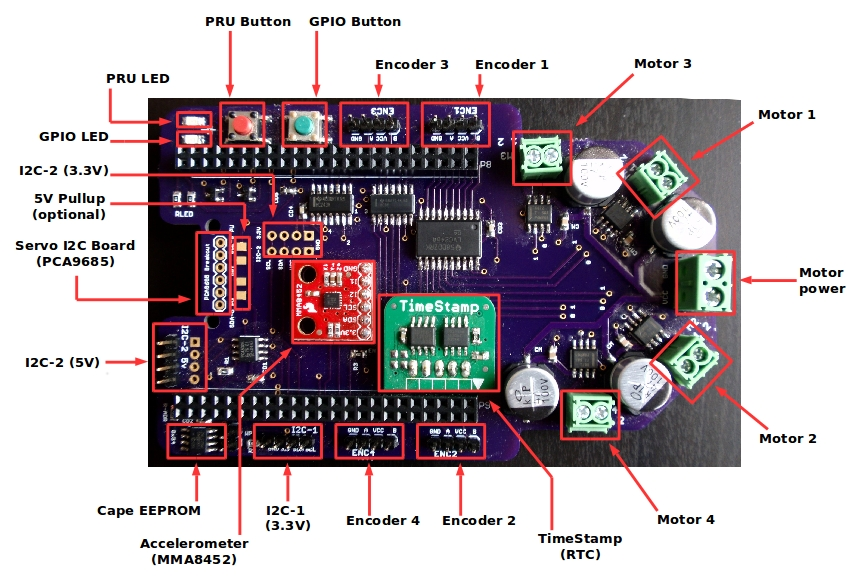
\includegraphics[scale=.4,keepaspectratio=true]{./images/BoardDiagram.jpg}
% \caption{SIUE Robot Cape}
% \label{fig:board_diagram}
%\end{figure}

%I put in the updated board diagram picture
\begin{sidewaysfigure}
 \centering
 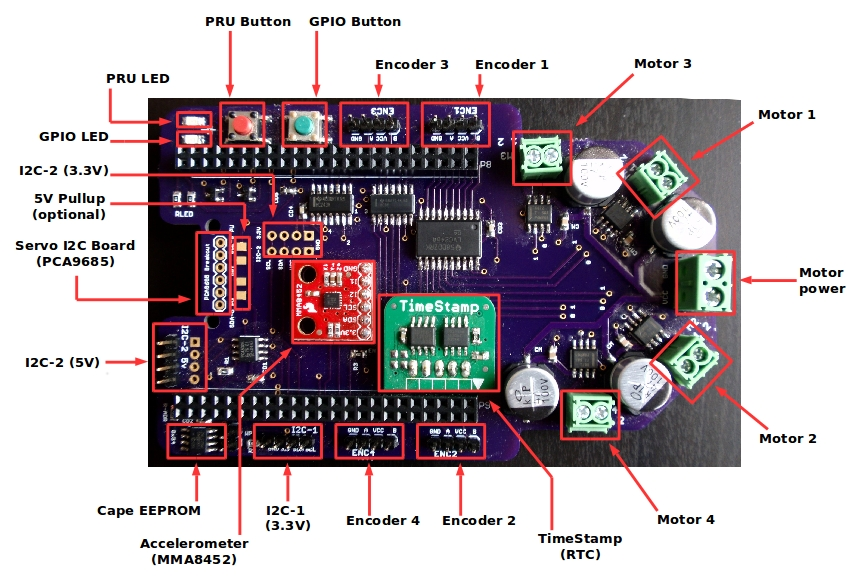
\includegraphics[scale=.7,keepaspectratio=true]{./images/BoardDiagram.jpg}
 \caption{SIUE Robot Cape}
 \label{fig:board_diagram}
\end{sidewaysfigure}


\section{LINUX Device Tree Overlay}

As just mentioned, the cape requires that an overlay be loaded into the Linux device tree to let the operating system know how to multiplex various pins in the system and load in the necessary drivers for the devices that are used by the board. The device tree is a structure used by hardware developers to describe hardware available to the system that is un-discoverable by the operating system ~\cite{eLinux-deviceTree}.  

In total the SIUE Robot cape uses 21 different pins on the BeagleBone Black in various pullup and pulldown configurations presented in Figure~\ref{tab:Pin_list}. The cape has an installed EEPROM chip on board with the board name and a description of the pins used by the board. The EEPROM memory map is defined in Figure~\ref{tab:EEPROM setup} which is taken from the BeagleBone Black System Reference Manual~\cite{BBB-SRM}.

\begin{table}[htbp!]
 \centering
 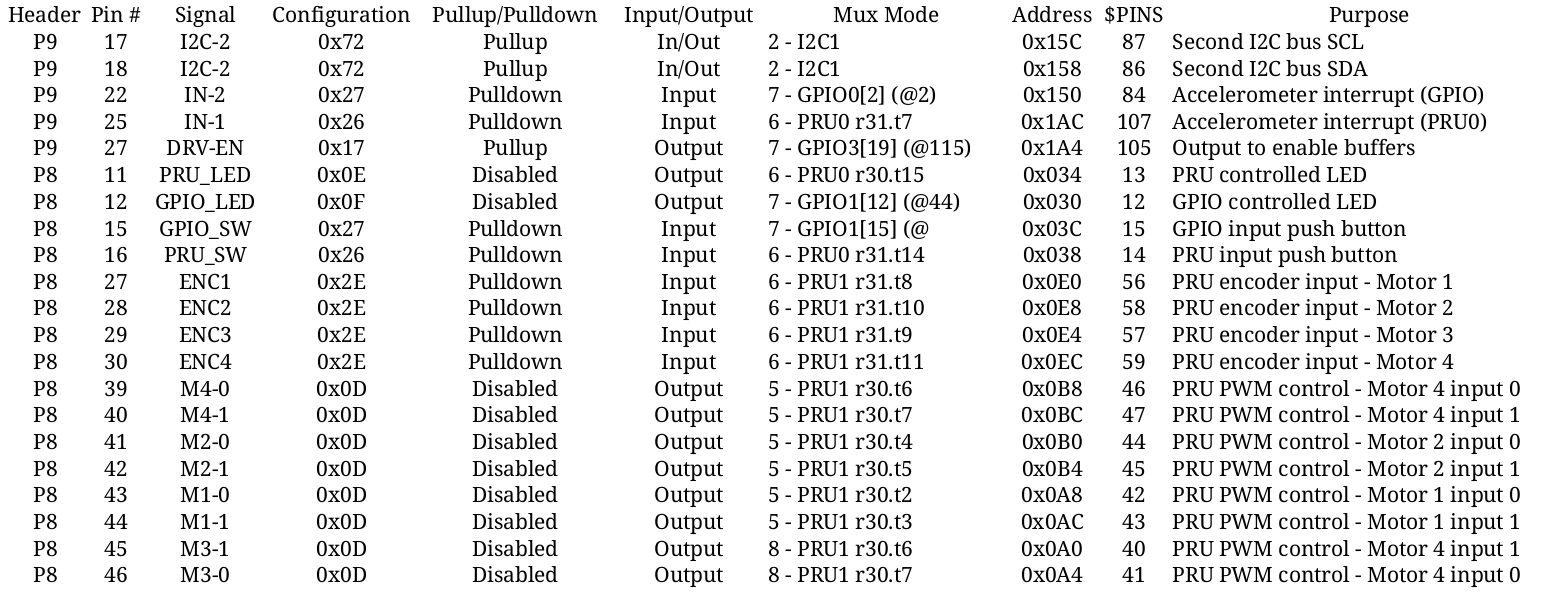
\includegraphics[scale=.3,keepaspectratio=true]{./images/Pinlist.png}
 \caption{BeagleBone Black Pins Used by SIUE Robot Cape}
 \label{tab:Pin_list}
\end{table}

\begin{table}[htbp!]
 \centering
 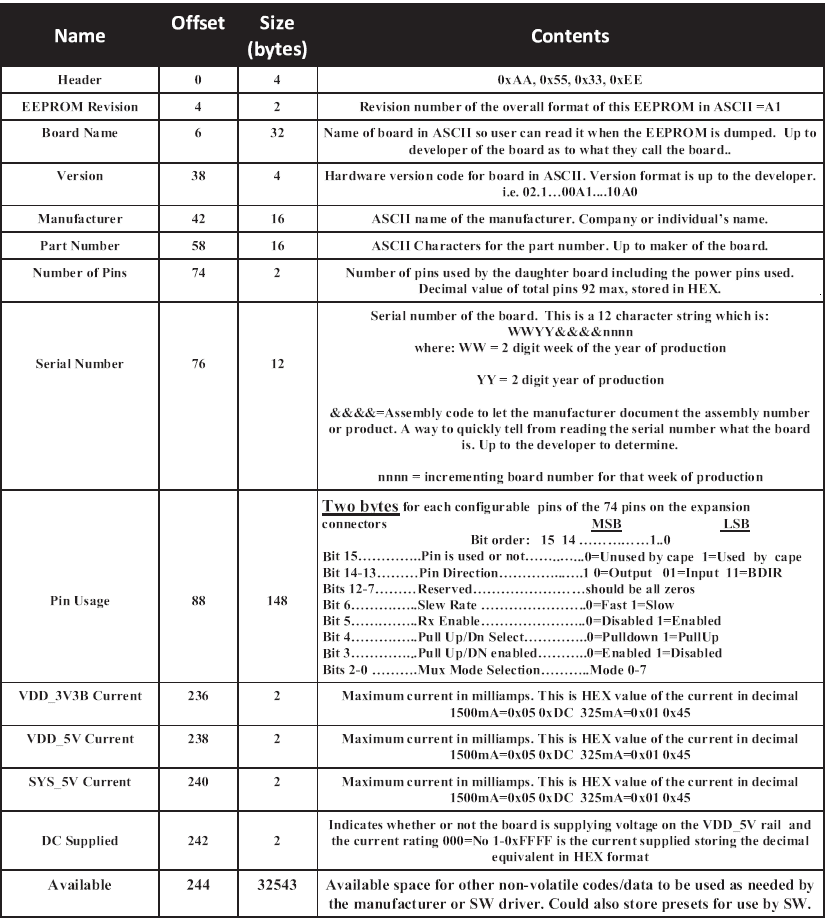
\includegraphics[scale=.75,keepaspectratio=true]{./images/eeprom_setup.png}
 \caption{EEPROM Memory Map}
 \label{tab:EEPROM setup}
\end{table}

This allows the board to be loaded at boot time by matching the correct compiled device tree overlay (device tree blob) located in the /sys/firmware folder. However, some changes need to be made to the uboot bootloader environment before this process can happen seamlessly. When a device tree overlay is loaded, that overlay has claim on the pins used by the different devices described by the overlay. 

A large portion of input/output PRU pins are included in the cape are claimed by the HDMI (video interface) and McASP (audio interface) normally and the HDMI overlay must be disabled. This is done by editing the uEnv.txt located in the /boot folder and uncommenting a line designated for removal if the HDMI and audio overlays are not needed. 

The last step requires editing the uBoot file itself so the board overlay is available to the bootloader. This is the result of a "chicken and the egg" problem with the BeagleBone’s EMMC (Embedded Multi-Media Card) which holds the actual Linux kernel and the bootloader which is running its own program to set up the boot environment. The EMMC is not actually native to the system and needs to be made available to the system through the use of an overlay. Overlays loaded on boot are only done once \emph{i.e.} before the unpacking of the kernel on the EMMC happens. So the SIUE Robot Cape device tree overlay needs to be in the bootloader’s firmware folder at boot time and not solely in the Linux firmware folder. 

This is fixed by using a script provided by the BeagleBone developers which uses \emph{initramfs-tools} to update the boot loader. A script must be placed in the initramfs-tools/scripts directory telling the tools to copy the firmware folder containing all the device tree blobs into the the firmware folder for the bootloader. Once this is done the bootloader now knows about the custom cape that it is attached to via the EEPROM and can load it properly.


\section{I2C Interface}

On the BeagleBone Black there are three available I2C busses but only two are accessible to the user on the P8-P9 headers.  These two buses I2C-1 and I2C-2 are claimed for use by the SIUE Robot cape. In the current Debian 3.8 kernel there is a slight confusion regarding the naming of these buses. In hardware schematics they are labeled I2C1 and I2C2. When these devices mount, their names become flipped I2C1 mounts in /dev as I2C-2 and I2C2 mounts in /dev as I2C-1.  

To reduce this confusion, they are labeled on the board with their I2C /dev names and henceforth in this paper they will be referred to as I2C-1 and I2C-2. The I2C-1 bus plays an important role in the loading of capes, because it is the bus that gets queried at certain addresses for attached EEPROMs and attempts to read the contents. 

There are only 4 addresses that are queried for custom capes. These 8-bit I2C addresses are 0x54, 0x55, 0x56, and 0x57. This means that only 4 capes can be loaded at boot at any given time but more capes can be loaded later by the user. I2C-1 is also where the on-cape I2C devices are located.  These I2C devices are the accelerometer breakout board and the real time clock with EEPROM (called TimeStamp) breakout board. 

A listing of addresses that are either taken or reserved is presented in Figure ~\ref{tab:I2C-1 List}. The I2C-2 bus is broken out in two different spots with two voltage logic levels (3.3 Volts and 5 Volts) and have no attached I2C devices. A level translator is provided on this bus.  It is the the PCA9306 which implements the Phillips specifications for I2C level translation and allows for devices that use 0 to 5 volt logic levels to talk to 0 to 3.3 volt systems such as the BeagleBone ~\cite{PCA9306}. 

On the board there are optional placements for SCL and SDA pull-up resistors, but often breakout boards using I2C have attached pullups so it may or may not be wanted. The final I2C device on the board is the PCA9685 breakout board which can control up to 16 servo motors. Since this device operates in a 0 to 5 volt logic environment, its connection to the level translator is on the high (5 Volt) voltage side.

\begin{table}[htbp!]
 \centering
 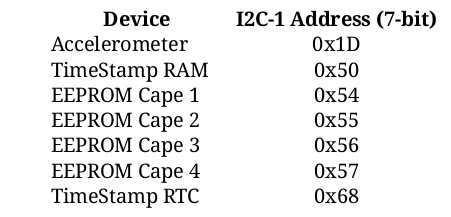
\includegraphics[scale=.5,keepaspectratio=true]{./images/I2C_addr.png}
 \caption{I2C-1 Addresses}
 \label{tab:I2C-1 List}
\end{table}

\section{H-Bidge Circuits}

\begin{figure}[htbp!]
 \centering
 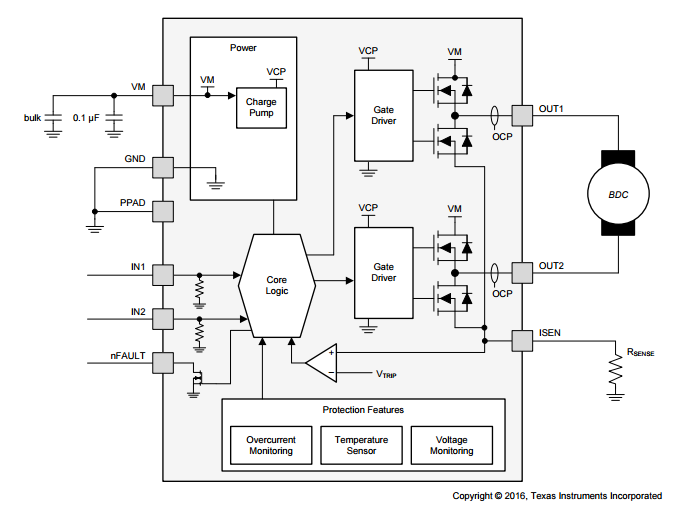
\includegraphics[scale=.85,keepaspectratio=true]{./images/DRV8872_block.PNG}
 \caption{DRV8872 Functional Block Diagram}
 \label{fig:DRV8872}
\end{figure}

The H-Bridge chosen for this application is a Texas Instruments DRV8872. This can be used as DC motor driver with a dual input control scheme, current sensing capabilities, and fault feedback. The H-Bridge circuit can drive 6.5 to 45 volts at 3.6 amperes peak in both a forwards and backwards rotation depending on the input signals~\cite{DRV8872}. 

This H-Bridge can also perform a hard brake or a slow decay (coast) based again on the input signals. Figure~\ref{fig:DRV8872} shows a logic block diagram of the chip, indicating some of the functionality of the chip~\cite{DRV8872}. There are a number of other features proveded by the DRV8872 shown in the block diagram such as overcurrent monitoring, temperature monitoring, and voltage monitoring which control the value of nFAULT which is the feedback pin on this chip. This functionality is not supported in the current version of this board and the pin is grounded. There is also an ISEN pin dedicated to current sensing, but this pin is grounded to achieve the maximum peak current possible. 

Physically, the chip comes in a 8-SOIC package with an extra pad on the bottom for thermal relief to a ground plane, which is dubbed the PowerPAD by Texas Instruments. This chip was mostly chosen for its small form factor and high current properties. In fact, the chip is physically smaller than the 47 $\mu$F bulk capacitors in parallel to it. 

On the board the input signals are driven by an 8-bit buffer and connected to motor power through wide traces via the power supply connection labeled "Motor Voltage" in Figure~\ref{fig:board_diagram}. Beneath the outcropping section is the ground pour which has to be at the same ground potential as the digital side of the board. To help prevent potential surges of power crossing over to the digital side, two ground pours were created and thin connections made between making them the same potential but restrictive in a high current sense.  

Large bulk capacitors are used along with smaller decoupling capacitors to help prevent fluctuations in power when the motors are active. The final output signal for these drivers are the individual motor outputs labeled in Figure ~\ref{fig:board_diagram} which are meant for the two wires of a DC motor or one drive pair for a stepper motor.

\section{Buffers and XOR Gate}

This board comes with two buffer chips: CD74HC243 (4-bit) and CD74HC245 (8-bit) and one quad XOR gate package (SN74HC86). These chips were added to handle situations where signals on boot or default values affect either the motors or the boot process of the BeagleBone. When the BeagleBone powers up some of the pins used by the PRUs in the final application are used to determine boot state. 

For example if one pin is pulled high on this bus it will attempt to boot from the SD card slot rather than the built in EMMC storage. Additionally the default state of these pins after the boot process may be left floating at voltages that would trip the logic levels of the H-bridges causing the motors to spin on boot and shortly after. 

The wheel encoders suffer from a similar issue. If a pin is to be an input during the boot process but it is attached to an encoder there is a chance for it to be high which in turn could interfere with the boot process. To address this situation buffer chips are used so that when the BeagleBone is in a state that would not require pin outputs or inputs, the buffers keep the system side in a high impedance state when not used.  In this way the H-bridges will never see an errant voltage level without being set properly first and the encoder input pins would not see a signal unless they were ready to. 

The high impedance state is controlled by a GPIO pin that is pulled up to 3.3 volts. During boot this makes the voltage high enough to trigger the high impedance state on the buffers and only by setting the GPIO pin to logic low state (\emph{i.e.} 0) can the buffers be activated. The 8-bit buffer controls the H-bridges by passing along the output of the PRUs and the 4 bit buffer handles passing the encoder signal to the input of the PRU after being handled by the quad XOR gate.

\begin{figure}[htbp!]
 \centering
 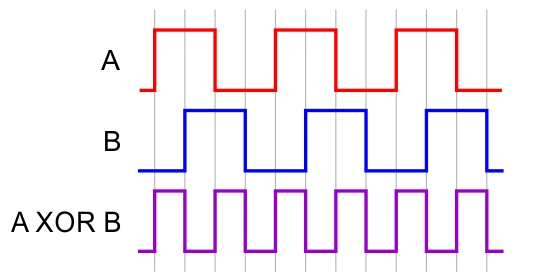
\includegraphics[scale=2,keepaspectratio=true]{./images/encoder.jpg}
 \caption{Encoder Waveforms Using XOR Gate}
 \label{fig:Encoder_wave}
\end{figure} 

The quad XOR gate receives the signal from the motor encoders and passes it to the 4-bit buffer chip. The role of the XOR gate is twofold: (1)  provides the ability to effectively read a pair of quadrature encoder signal without the actual need for inputs for both the A and B channels, and (2) provides a means of level translate a 5 volt signal to 3.3 volts. 

Quadrature encoders are fairly common. The term implies that there are two signal in the form of square waves with a 90 degree phase shift between them. As the motor rotates and depending on which channel is read first, the rotation direction can be determined. However, if the motor direction is being controlled it becomes a pointless feature and just ends up taking an extra input to get full resolution of the encoder ticks. Using an XOR gate for the two input channels (A and B), full resolution of the encoder ticks can be achieved as there will be a pulse for every positive edge of the A and B signals as shown in Figure~\ref{fig:Encoder_wave}~\cite{encoder}. 

The input pins on the SN74HC86 are up to 7 volt tolerant and their output voltage level is determined by the supply voltage. By hooking up the supply voltage to 3.3 volts, the SN74HC86 performs level translation. It accepts 5 Volt signals and translates them to 3.3 Volts. 

\section{Real-Time Clock}

The \emph{TimeStamp} board was developed by Dr. Noble of SIUE for a water sensor application but works well as a general RTC  (Real-Time Clock) breakout board. \emph{TimeStamp} also comes equipped with a 16 KByte FRAM (Ferro-electronic RAM) chip for storing constants if necessary and a battery holster for a 3 volt BR1225 coin battery to continue RTC operation without an external power supply. 

The RTC used in this module is a DS3231 clock module made by Maxim which has a time accuracy of $\pm$0.432 seconds a day and leap year compensation up until the year 2100 ~\cite{DS3231M}. Information is retrieved and updated through typical I2C operations. This board was added later in the design and was also chosen because of its small form factor and how easy it was to integrate into the cape design. 


\section{Accelerometer}

Typical accelerometers available on the market are small devices made to be utilized in cell phone applications and as a consequence are incredibly small and hard to hand solder. Using a breakout board is very typical in these situations. A company called Sparkfun sells an I2C accelerometer breakout board using the MMA8452. It is a three axis accelerometer with two output interrupt signals that can be tied to a number of different events. 

The device has an output data rate ranging from 1.56 Hz to 800 Hz and user selectable full scales of $\pm$2g, $\pm$4g, and $\pm$8g as well as the options to output high pass filtered data or unfiltered ~\cite{MMA8452Q} data. The interrupt signal can be connected to a data ready flag, freefall alert, or even an orientation signal to name a few.  

On the board the INT1 and INT2 signals are connected to a PRU input and a GPIO input respectively. Currently they are unsupported in our software. The accelerometer is useful in a robot because it can potentially provide information on how it is orientated, the direction it is traveling in space, or if a collision has happened. When developing in the future such a tool can be used to supplement the encoder feedback by observing things like slippage.

\section{Servo Motor Controller}

As explained in Chapter 1, it is important that the cape support all three types of motors. In order to support servo motors, the board includes a place to plug in a 16-Channel 12-bit PWM/Servo Driver. The PCA9685 is available from \emph{Adafruit} at at a cost of about fifteen dollars.  The breakout board was selected because of its following features.

\begin{itemize}
\item
I2C-controlled PWM driver with a built-in clock, 
\item
5 Volt compliant, 
\item
adjustable frequency PWM up to about 1.6 KHz,
\item
12-bit resolution for each output \emph{i.e.} (for servos that means about 4us resolution at a 60 Hz update rate),
\item
configurable push-pull or open-drain output,
\item
and output enable pin to quickly disable all the outputs.
\end{itemize}

\section{User LEDs and Switches}

The SIUE Robot Cape also provides the user with 2 momentary (pushbutton) switches and 2 LEDs (Light Emitting Diodes). One LED-switch pair is connected to GPIO pins.  The other pair is attached to PRU fast I/O pins. The pair connected to GPIO pins can be accessed by either the PRU or by the ARM. The other pair is accessible only by PRU 1.

LEDs and pushbutton switches are some of the most rudimentary debugging tools and can be useful when a terminal is not available to the user. In past competitions, SIUE teams have had to implement a start button for the robot that would start the execution of the main program, and frequently blinking an LED is a required task which allows the judges to know when the robot has completed the competition or a specific task. 

For the switches, when pressed a 3.3 volt signal is connected to an input pin in a pull-down configuration. The LEDs are controlled by N-Channel MOSFET (BS-223) whose gate is connected to an output pin, and the LED in series with a resistor are placed between the 3.3 volt supply and the drain. When the associated output pin is brought high, the MOSFET conducts and current flows from the drain to the source which in turn causes current to flow through the LED, thereby turning it on.


\section{Schematic and PCB Layout}

The schematics for the SIUE Robot Cape are presented in Figure~\ref{fig:Schematic_1} and Figure~\ref{fig:Schematic_2}. Each IC in the schematic has its own decoupling 0.1$ \mu$F capacitor to prevent supply voltage fluctuations. The printed circuit board (PCB) layout is highlighted in Figure~\ref{fig:Layout}. Schematic entry and PCB layout was performed using EAGLE 7 software from \emph{CadSoft Computer}.

\begin{sidewaysfigure}[htbp!]
 \centering
 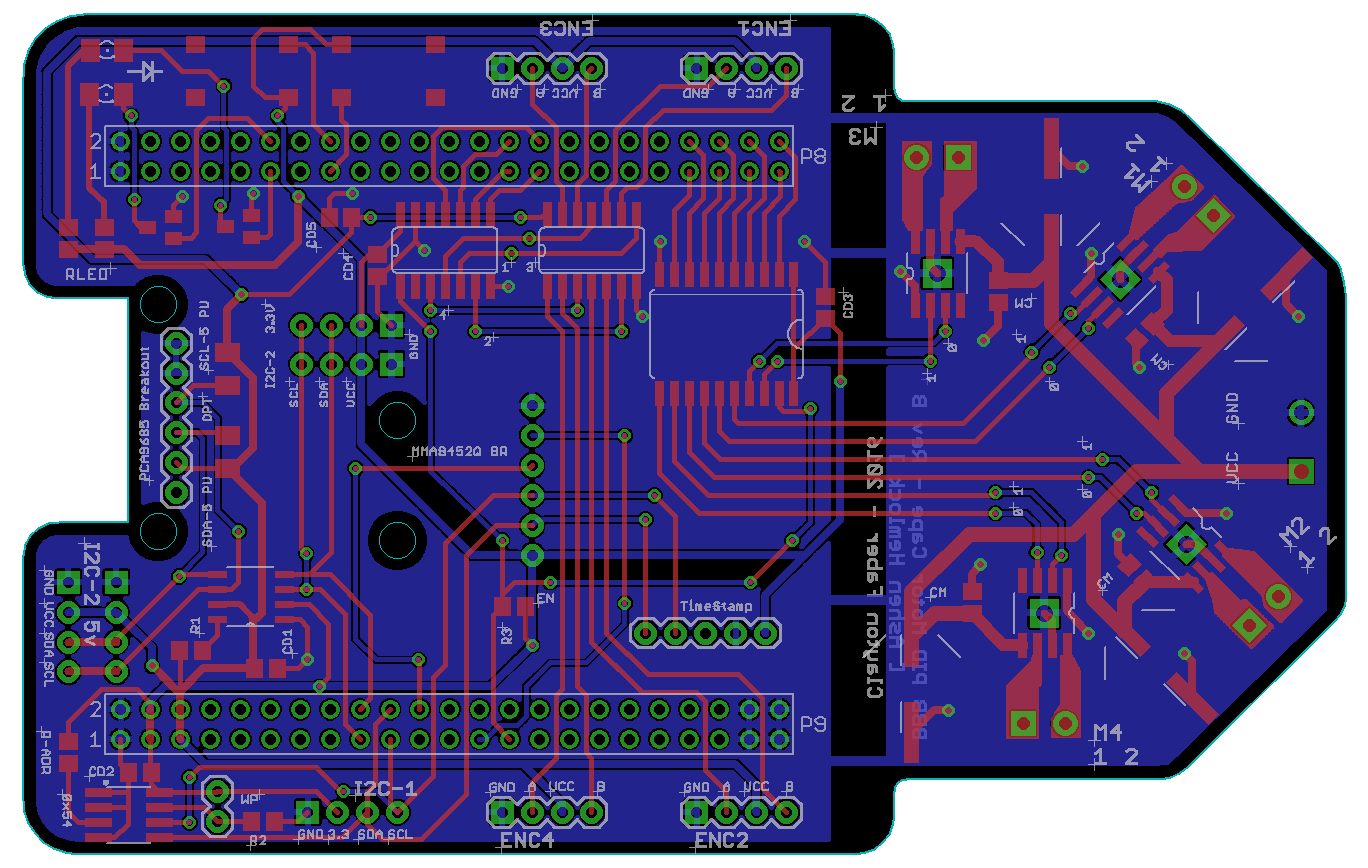
\includegraphics[scale=.5,keepaspectratio=true]{./images/layout.PNG}
 \caption{PCB Layout of SIUE Robot Cape}
 \label{fig:Layout}
\end{sidewaysfigure}

\begin{sidewaysfigure}
 \centering
 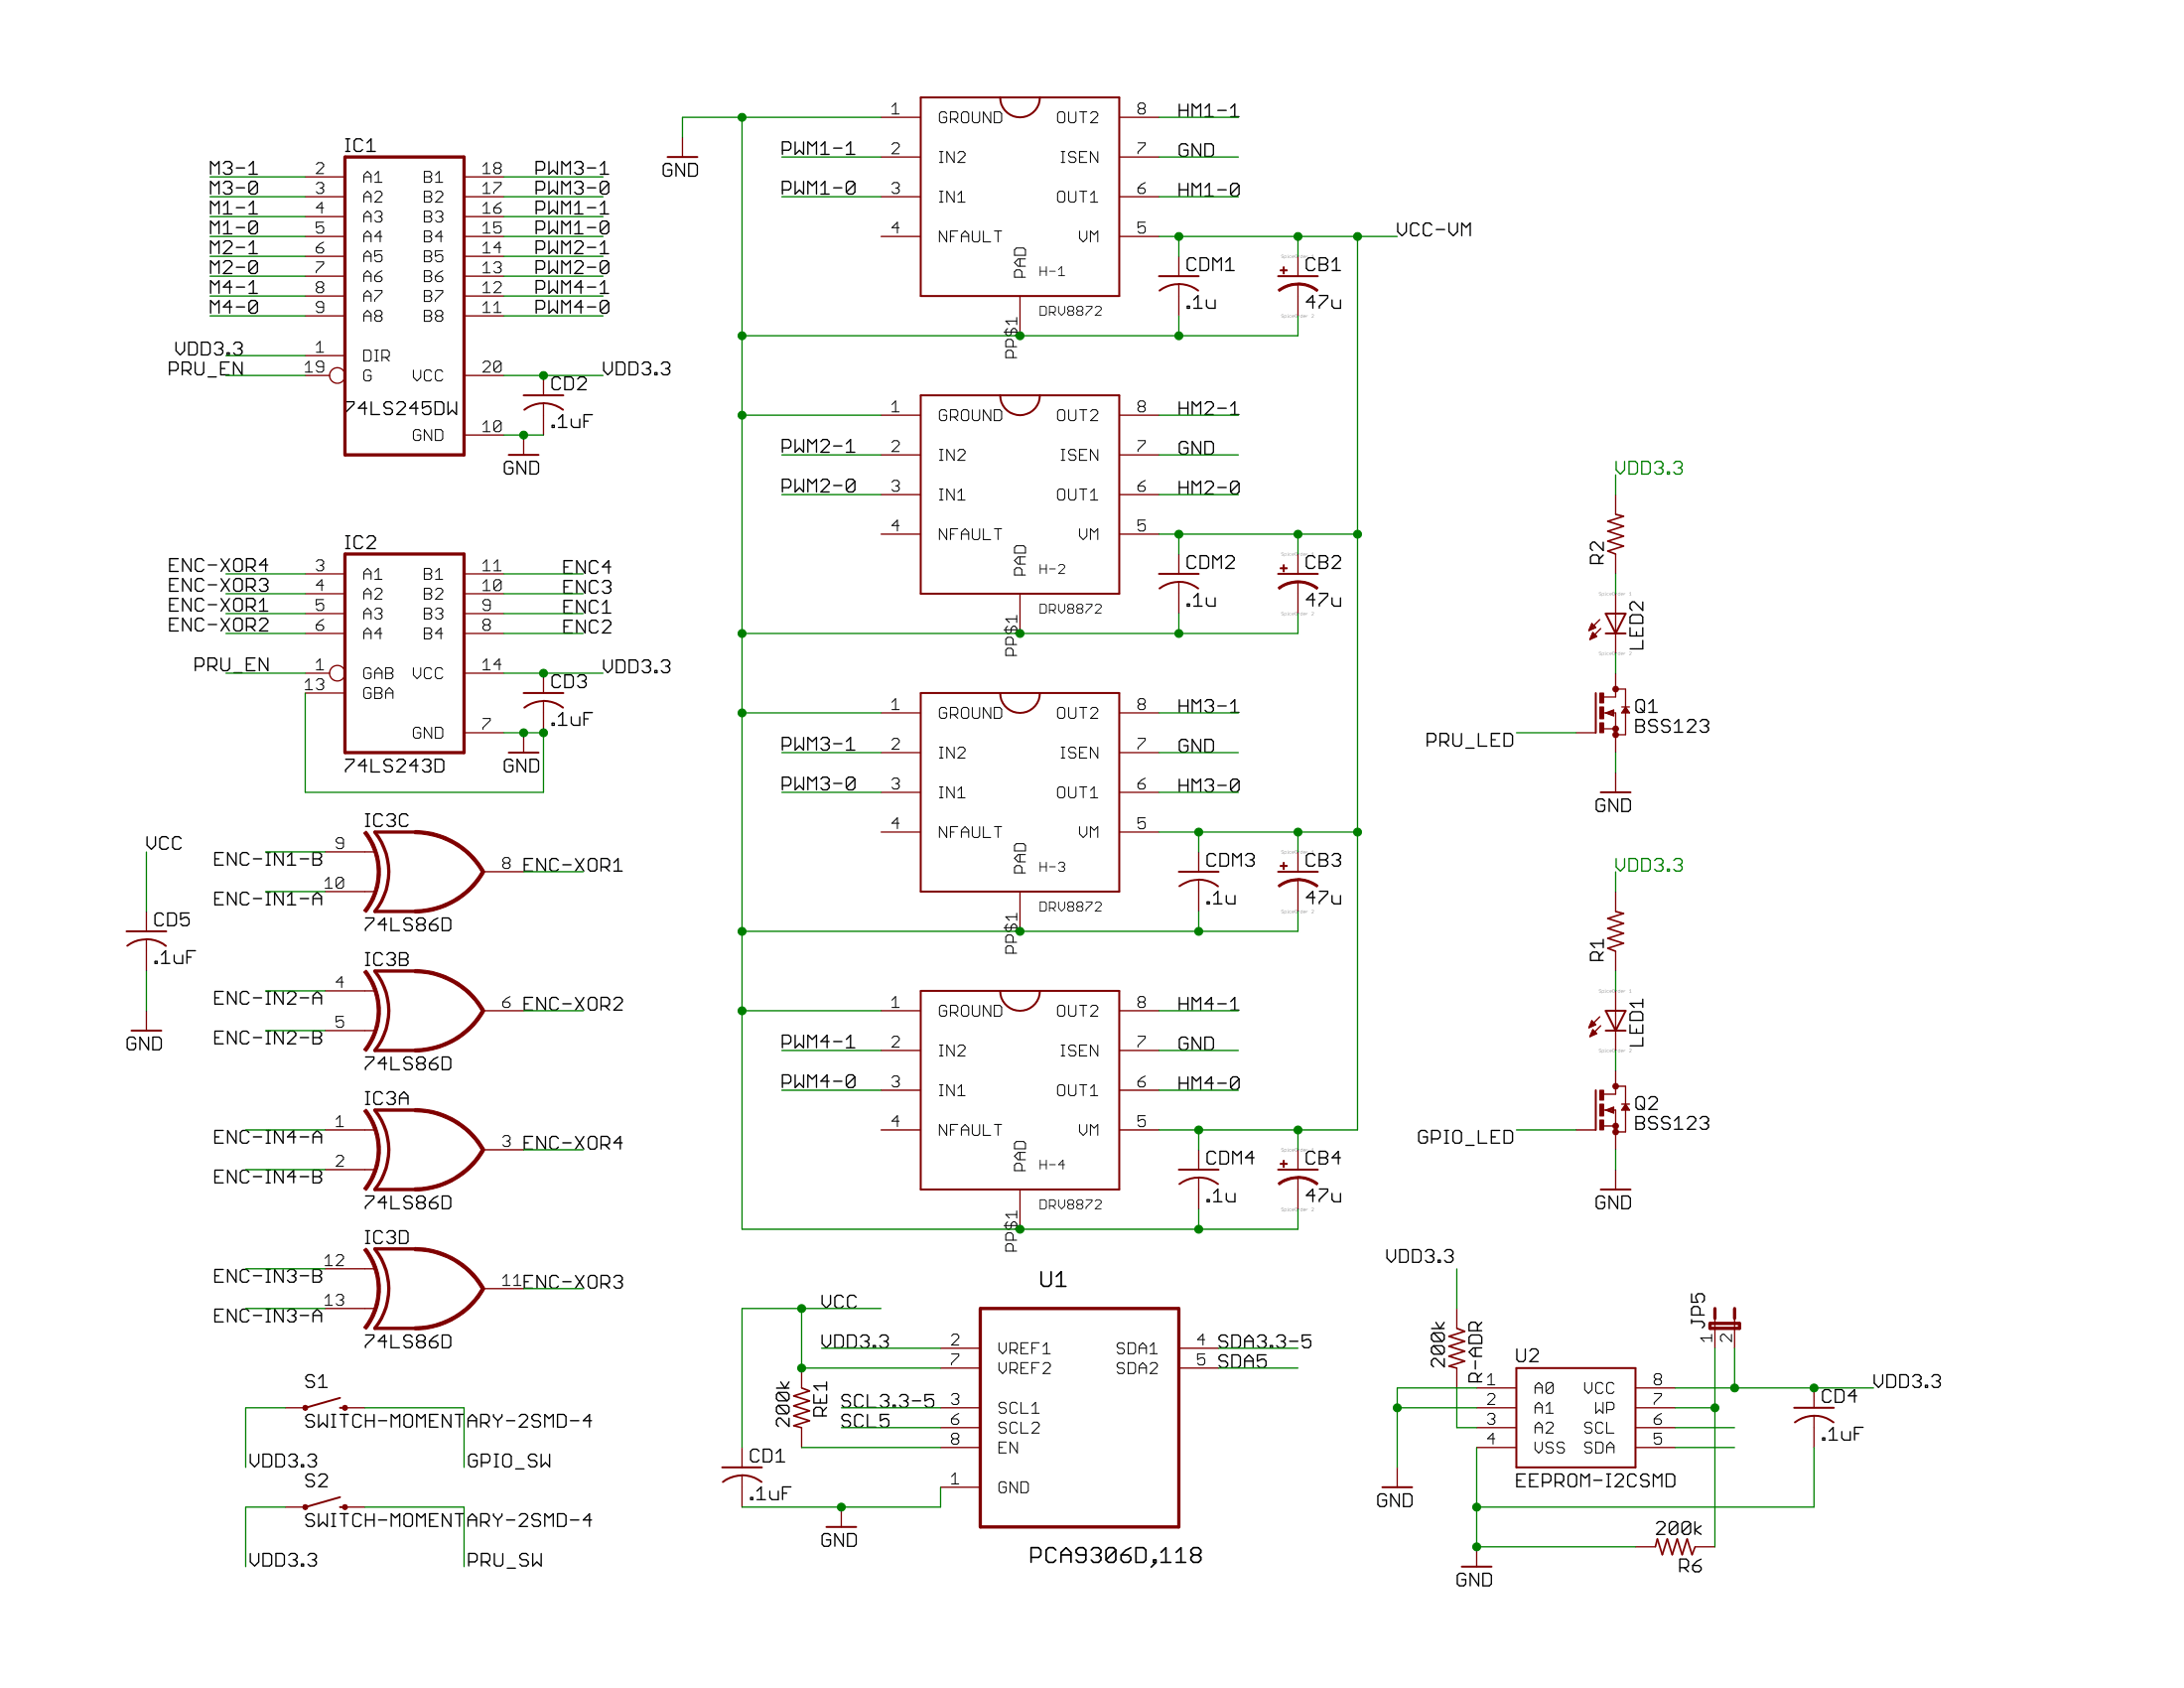
\includegraphics[scale=.25,keepaspectratio=true]{./images/schematic_1.png}
 \caption{Schematic of SIUE Robot Cape (1 of 2)}
 \label{fig:Schematic_1}
\end{sidewaysfigure}

\begin{sidewaysfigure}
 \centering
 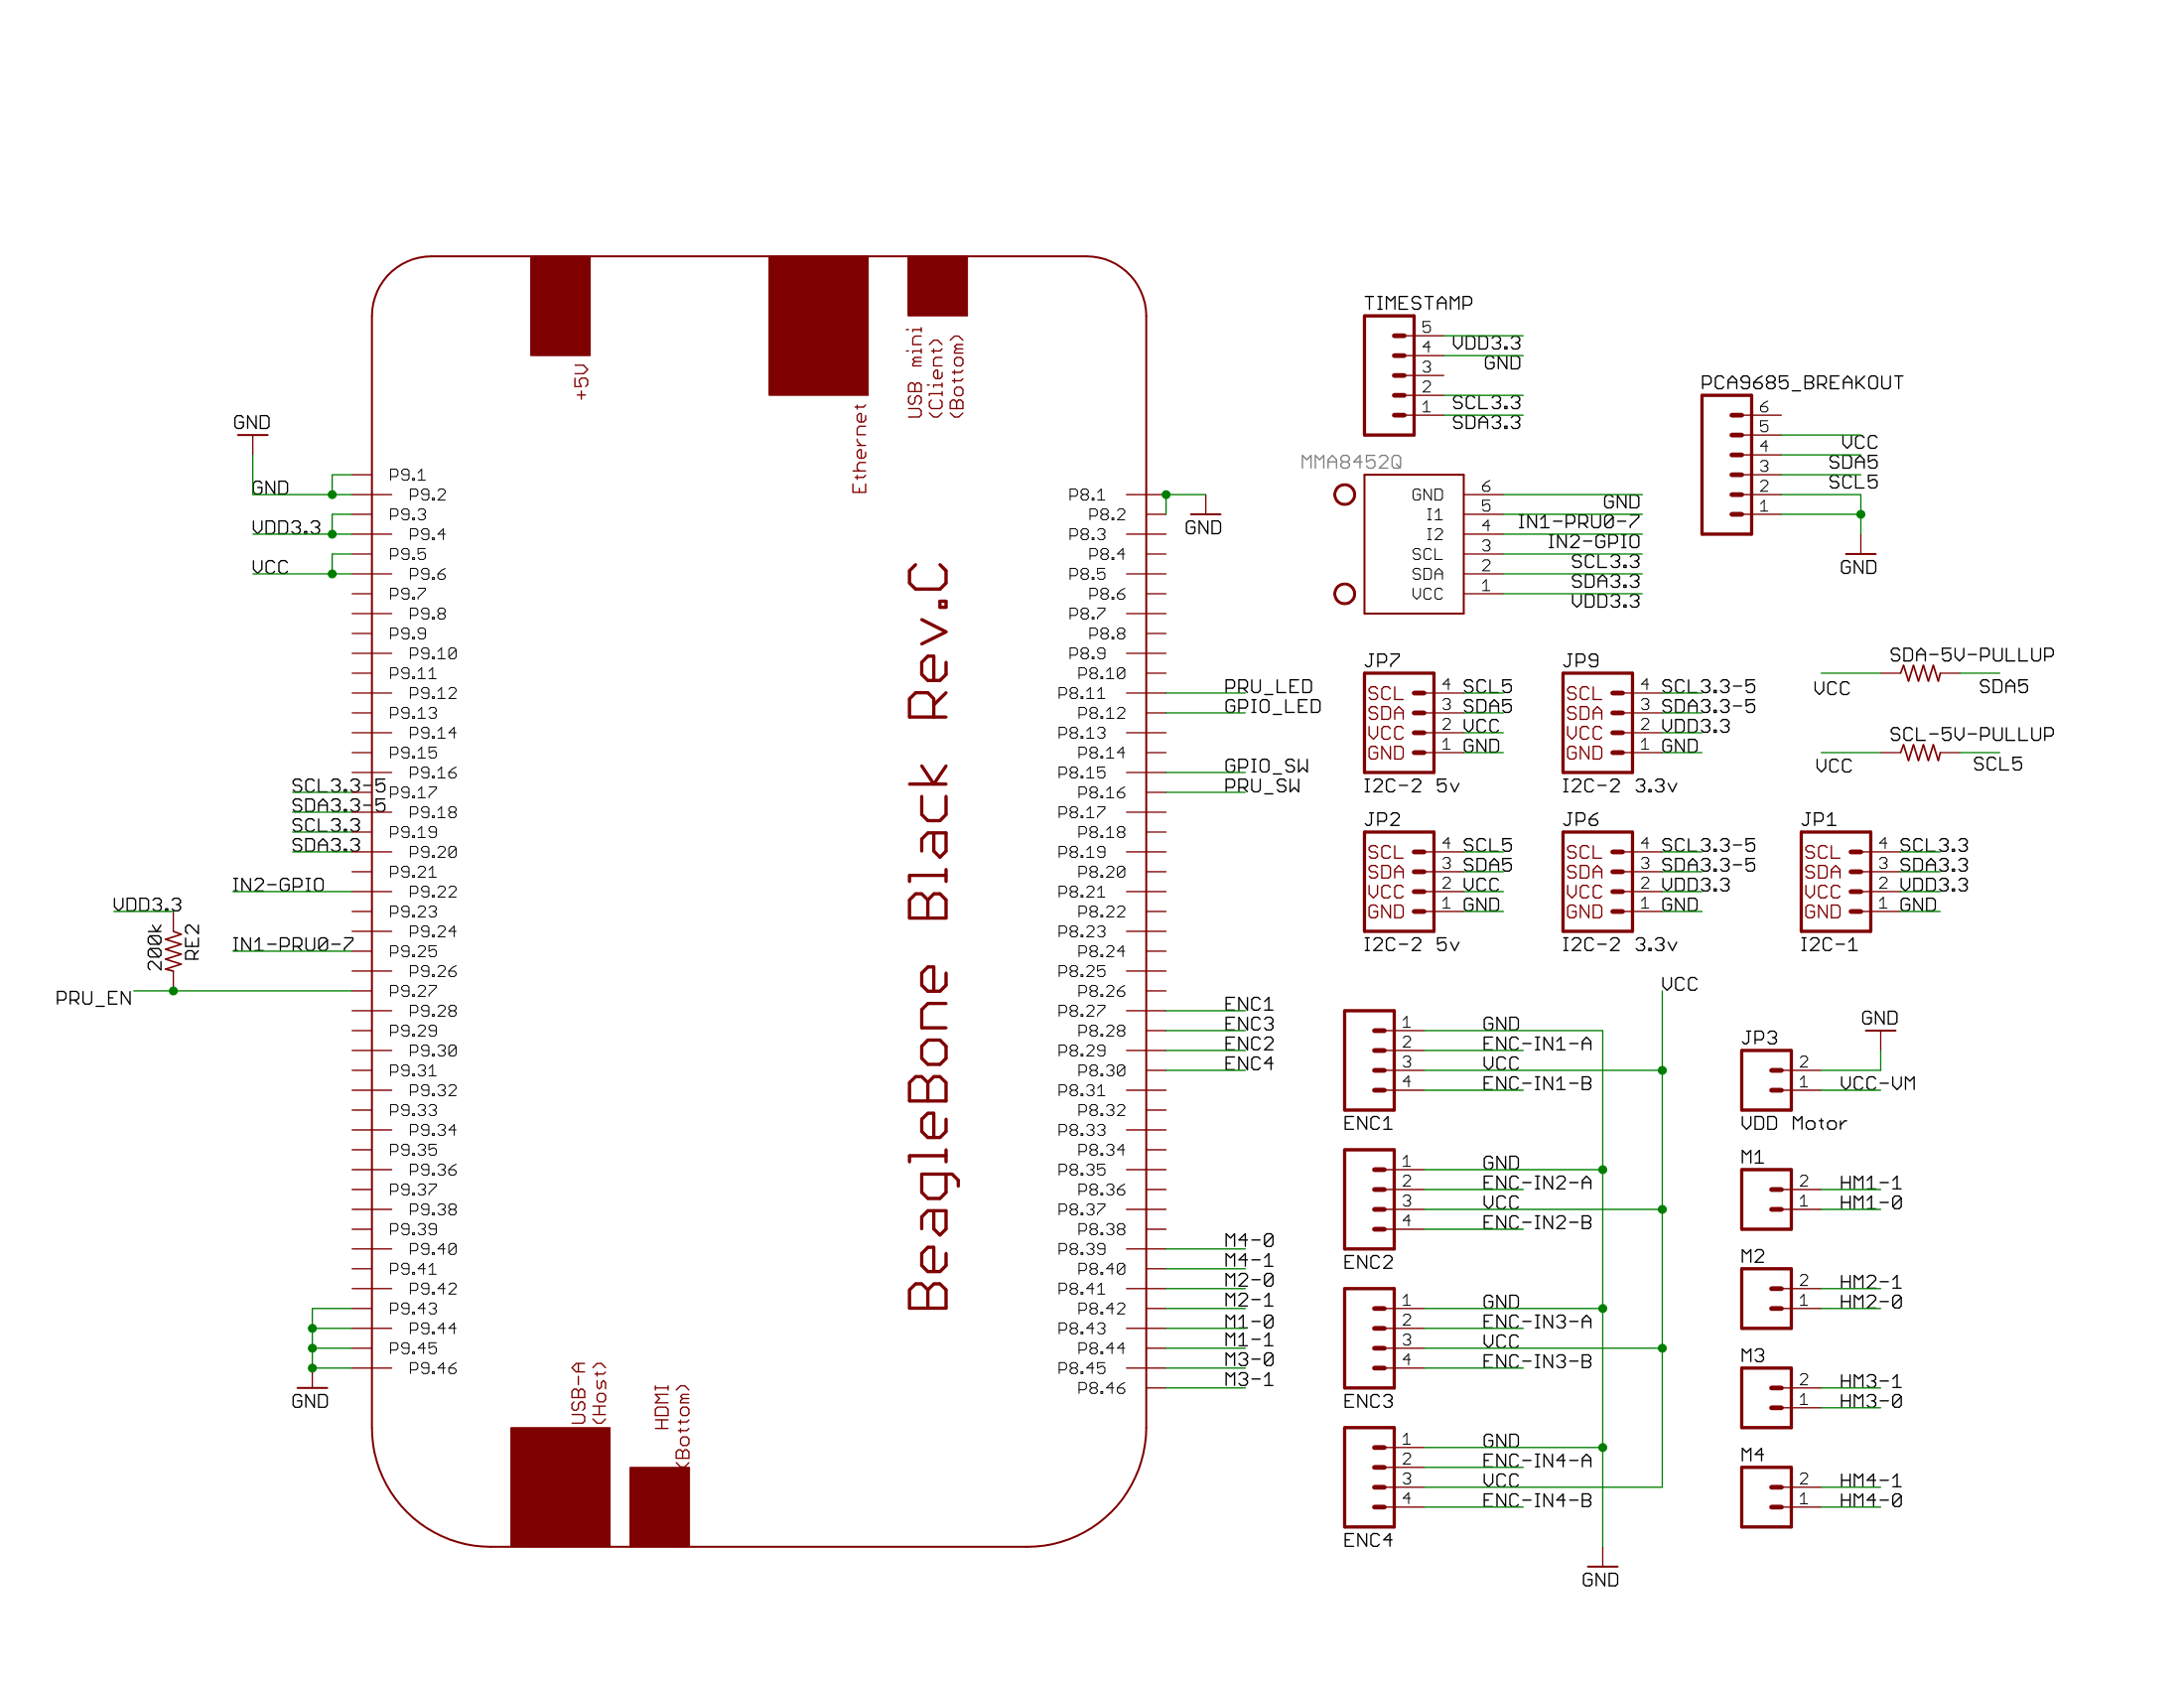
\includegraphics[scale=.25,keepaspectratio=true]{./images/schematic_2.png}
 \caption{Schematic of SIUE Robot Cape (2 of 2)}
 \label{fig:Schematic_2}
\end{sidewaysfigure}


\chapter{ELECTRICAL LEVEL DESIGN}

\section{Software Design Objectives}

The program controlling a robot is as (and perhaps even more) important than the robot frame itself, and while the cape is an important piece of hardware, it cannot drive the motors without some type of control program. In this chapter a general overview, software design objectives, algorithms, and software routines used to control a pair of DC motors will be discussed.

As already described, the BeagleBone Black possesses \textbf{two} 32-bit RISC cores, called PRUs (Programmable Real-time Units), each with their own data and instruction memories and also with direct access to the P8 and P9 headers. Moreover, each PRU has access to a 32-element register file with just two of the registers \emph{reserved} for GPIO and system status use (\emph{i.e.} there are 30 for general use).  Each PRU can access 8 KB of program memory and 8 KB of data memory. They also have access to a 12 KB block of shared memory which can be used by both PRUs as well as by the ARM core.

The two processors can run programs independent of each other and independent of the ARM. All processing of motor control signals will be directly handled by the two PRUs in a master-slave relationship. The ARM requests movement by setting values in shared memory and can then monitor a specific location in the shared memory to determine when the command has completed. All three processors (PRU10, PRU 1, ARM) use the shared memory as a way to communicate through the use of command and data words. 

A DC motor controller needs a way to handle encoder feedback, perform calculations based on that feedback, and then in turn control the PWM duty cycle for the H-bridges which directly drive the motors. For a two-wheeled robot, we will see that this will entail implementing 3 PID loops.

Each PRU runs at a clock speed of 200 MHz (\emph{i.e.} a 5 nanosecond instruction execute time) and while this is quite fast it would not guarantee enough time to do both calculations and handle the real-time applications of the PWM and encoder feedback for two motors. To solve this problem, it is advantageous to break up the workload between the two PRUs: one (PRU 0) doing calculations while the other (PRU 1) provides a direct interface to the SIUE Robot Cape hardware. The unit directly interacting with the hardware needs use its clock cycles efficiently and is therefore best programmed in assembler. 

There is 12 KB of shared memory that can be used by all three processors and sits on the PRU’s bus for their direct access without the need to access ARM system RAM which would require further processor time. Design objectives for the ARM system will be covered in detail in the following chapter, but it is important to note that its role in this design is to issue commands to PRU 0, place configuration data in memory, and start the process of motor control. PRU 0 in turn communicates with PRU 1 which controls the hardware on the cape.

\section{PID Algorithm Overview}

While PID algorithms have been discussed at length in other publications, a brief overview will be presented. A PID controller is used to maintain a certain setpoint through calculations based on a feedback signal. PID is an acronym of three separate control algorithms: proportional, integral, and derivative using a feedback signal as an input. The three partial terms are calculated and then their sum determines the output. 

The three PID loops have their own gain values which are used to tune the loop. In this application we wish to control two DC motors and as such there are three PID loops in use. Two loops are set up to control each individual motor's velocity and a third differentially controls the two motors' velocity setpoints. A system block diagram depicting the two slave loops and the master loop is shown in Figure~\ref{fig:PID_Dia}. 

\begin{figure}[htbp!]
 \centering
 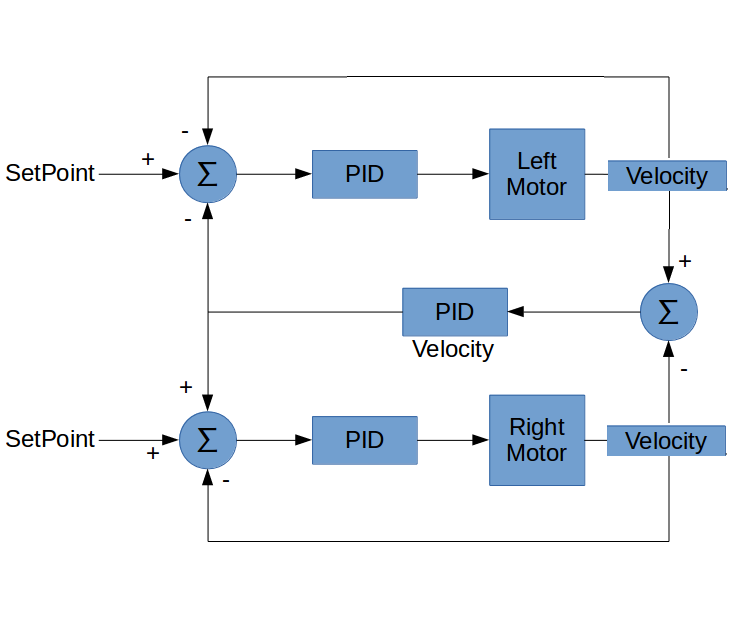
\includegraphics[scale=.45,keepaspectratio=true]{./images_ch3/PID_diff_flow.png}
 \caption{Block Diagram of PID Control Used in Differential Drive Design}
 \label{fig:PID_Dia}
\end{figure}

This scheme helps get the most out of a differential drive machine and helps compensate for disparities between DC motors~\cite{PID_Diff}. By having a master control loop that differentially drives the wheels, the robot can account for errors during travel. For example, if one wheel happens to encounter a carpet causing it to decrease in velocity the master PID control loop would cause the wheel on the carpet to spin at a faster rate in order to overcome the additional resistance presented by carpet and at the same time the wheel not on the carpet would slow down at a proportional rate to attempt to keep the robot moving in a straight line. 

This also comes in handy when dealing with the step response of DC motors. DC motors are not created equal and as a consequence their inductances do not always match. Because of this, one motor may react quicker than the other when starting from a dead stop and cause the robot to become misaligned. With the third PID loop in place, the PID loop will observe that one wheel is spinning faster than the other and in turn will attempt to solve the problem. 

The input of the PID controllers driving the two DC motors is the error (\emph{i.e.} e(n)) between the setpoint value and the encoder count observed during a single sample period. The setpoint value is the velocity of the motor or more specifically the number of encoder tics that should occur during a single sample period for the corresponding velocity. The third PID loop's input is the difference in wheel velocities. The setpoint for the third loop in the current implementation is zero so as to ensure straight-line movement but this need not be the case. One could drive the differential velocity to something other than zero which would cause the robot to follow an arc. In this way, arbitrary paths could be followed.

The "differential" form of the PID algorithm (Equation 3.1) is used in this work ~\cite{PIDctrl}.  The next PWM output is computed by taking the current output and adding a "delta" which is calculated using the PID constants. The "past" error is e(n-1) and the "past-past" error is e(n-2).  The PID constants are $K_p$, $K_i$, and $K_d$. This results in a much simpler algorithm, only requiring a couple lines of code with just a few fixed-point math operations.
\begin{eqnarray}
pwm(n) &=& pwm(n-1) + \Delta(n) \\
\Delta(n) &=& \Delta_p(n) + \Delta_i(n) + \Delta_d(n) \nonumber \\
\Delta_p(n) &=& K_p \cdot e(n) \nonumber \\
\Delta_i(n) &=& K_i \cdot \left[ e(n) - e(n-1) \right] \nonumber \\
\Delta_d(n) &=& K_d \cdot \left[ e(n) - e(n-1) + 2 \cdot e(n-2) \right] \nonumber
\end{eqnarray}

Fixed-point arithmetic is used rather than floating-point due to the large overhead associated with floating-point calculations and the amount of program space it takes up.  Values are calculated in a Q6 fixed-point format (6 fractional bits). By using a Q value of 6 we ensure a very high dynamic range (150 dB) but yet retain sufficient fractional information to keep the errors within reasonable bounds. 

The conversion between fixed- and floating-point representation occur within the ARM program which places the fixed-point values in shared memory for the PID controller to use. It should  be noted that the Q-value can be easily changed since it is defined in the fixed-point include file.

\section{Shared Memory Map}

Each program relies on shared memory for accessing values set by other processors. In the case of PRU 1, PWM values are read and encoder values are written to shared memory. PRU 0 reads constants for us in calculations and sets status flags in the movement process for the ARM core to read later. All three devices have to agree on how the memory is structured with both single word values and structures being maintained in it. This task is achieved through the mem.h file where, along with other constants and aliases, a shared memory structure is defined.

The mem.h file exists as one file in the project with symbolic links in both the PRU and ARM compilation directories. The ARM and PRU 0 coompilers think they have their own copy of the file but in reality there is only one copy which makes editing simple because a change in one file causes the change to show up for everyone with a link to it. 

The mem.h file has a structure definition called shared\_memory\_t. Both the ARM and PRU 0 code define a pointer to this shared memory structure and its value is set equal to the start of shared memory. When a structure is created in C, memory is allocated based on the data length of the structure. When accessing a certain value in a structure using a pointer, the C compiler takes care of the offset for the user. 

When the ARM program sets a value in the shared memory structure, PRU 0 reads it in the same way the ARM core wrote it because they share the definition of the structure. In Figure~\ref{fig:Shared Memory} the listing of the shared memory structure is defined on the left which contains all the values and structures used by all three processors. Because it does not have access to the pointer and structure declarations, the memory locations PRU 1 uses are placed at the beginning of the structure. This makes determining the offset easier. After PRU 1 values are defined, other structures and flags are created to help organize data. The structures available in shared memory are shown in Figure~\ref{fig:Shared_Memory}. 


\begin{figure}[htbp!]
 \centering
 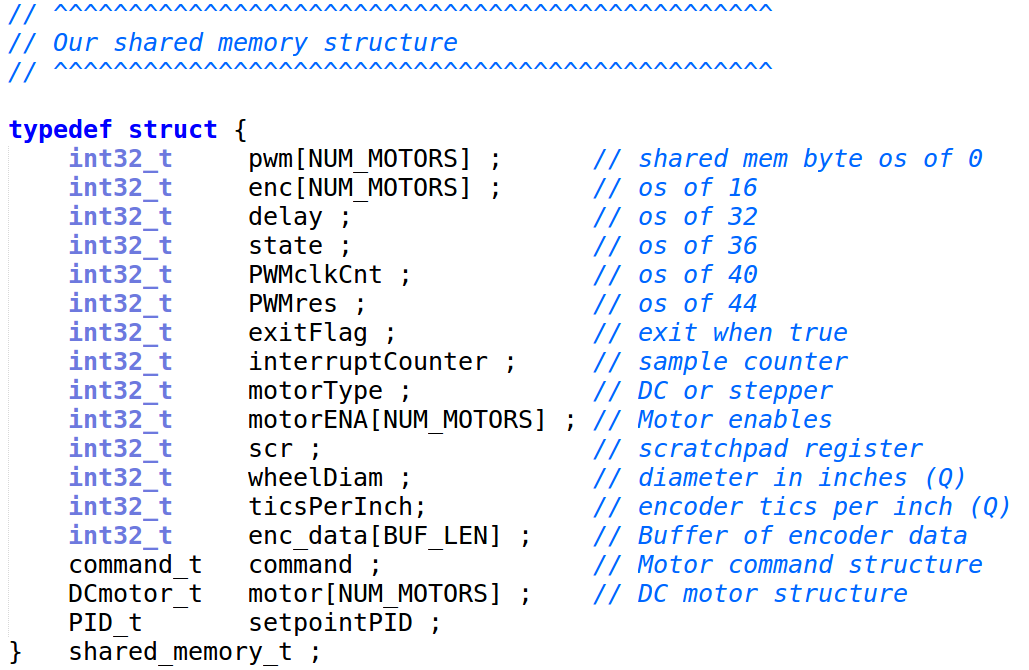
\includegraphics[scale=.35,keepaspectratio=true]{./images_ch3/sharedmemory-define.png}
 \caption{Shared-Memory Map}
 \label{fig:Shared_Memory}
\end{figure}


\section{PRU 1: Hardware Interface}

PRU 1 was chosen to directly interface to the SIUE Cape hardware due to its access to input/output pins on the P8 header. We require 8 outputs for the H-Bridge motors and 4 inputs for the encoder feedback. Along with these real-time signals, PRU 1 must also act as the timekeeper letting PRU 0 know that the sample period is complete and that it is time to calculate new PWM outputs. As a result of these real-time constraints, PRU 1 is programmed in assembly code in order to keep track of execution time which, per instruction except memory access, is 5 nanoseconds. Fortunately, in order to make things easier for programmers the assembler allows for the use of "macros" and "defines" in the code through the use of header files.

In the header file for PRU 1, pru1.h, there are a list of defines and macros which makes the program, pru1.p, easier to understand. Because the PRU system has a large number (32) of registers it was best to use defines to create an alias for each register and give it a specific purpose. These assignments are given in Figure~\ref{fig:PRU1_reg}. 

The motor control bits are defined first which are part of the output register, r30, and have a “.t\# ” following them to define the bit number. These are not in numerical order in order to make the layout of the board easier by following the numbering of the H-Bridges. As an example, r30.t1 corresponds to M3-1 which is connected to the output pin P8.45 which is in the very last row of P8 connector which is connected to the corresponding H-bridge on the top of the board as pictured in Figure~\ref{fig:board_diagram}. 

Moving down the list, a \emph{nop} alias is defined which is used in NOP operations as a means of effectively "stalling" the processor. Next, the registers that will hold the encoder and PWM values are defined.  The encOLD, encNEW, and encEDGE registers play a role in reading encoder ticks by saving values from the input register, r31, which will be described in more detail shortly. 

Next, a set of 6 GPIO registers are listed which can be used to access the Linux space GPIO pins that are connected to the motor cape. These can be used for debugging purposes. The next three are registers that hold control values. The register pwmResReg holds the maximum value corresponding to the resolution of the PWM signal. For example, an 8-bit PWM signal would mean that this register holds an unsigned value of 255. The stateReg acts as a way for the PRU 1 and PRU 0 to communicate without solely relying on interrupts as well as the control of the motor spin direction. 

Certain bits are designated as flags and are used to let PRU 1 know what mode it is in and if it needs to stop or start. Similarly a section of the register is used to designate how the motor will spin and are also is used to start the PWM outputs. This is achieved by loading the bottom byte of stateReg into the bottom byte of r30, the output register, effectively starting the on timer for the PWM signal. The delayClkCnt register holds the value corresponding to the number of PWM cycles making up a PID sample period. 

The i and j registers are used for counting the iterations of the two loops: PWM and sample period. Lastly, aliases are given for the different registers that hold the memory address values which are used as pointers for the different locations in memory. Although there are more defines listed in the appendix, these give the general overview of what kinds of values are in use. These defines are used in the macros also defined in pru1.h, a listing of important macros are available in tables ~\ref{Tab:PRU1_Macro1} and ~\ref{Tab:PRU1_Macro2} with a short description of their usage and function. Together these are used in pru1.p and make up the main body of the program.

\begin{figure}[htbp!]
 \centering
 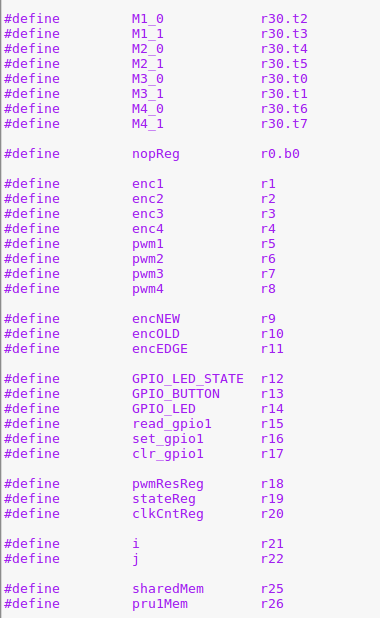
\includegraphics[scale=.75,keepaspectratio=true]{./images_ch3/pru1_define.png}
 \caption{PRU 1 Register Aliases}
 \label{fig:PRU1_reg}
\end{figure}

\begin{table}
    \begin{tabular}{ | c | p{11cm} |}
    	\hline
	Macros & Usage and Description  \\ \hline
	
	\multirow{2}{*} {get\_state} & Usage: get\_state \\& Update the status register value in pru1. b0 contains wheel control information, while b1-2 contain flag bits.
	Can be updated in shared memory from PRU0 or ARM \\ \hline

	\multirow{2}{*}{read\_clk\_cnt} & Usage: read\_clk\_cnt \\& Reads in the number of PWM cycles to run before interrupting PRU0. \\ \hline

	\multirow{2}{*}{read\_pwm\_res} & Usage: read\_pwm\_res \\ & Reads in the pwm maximum count from sharedMemory. Either 255 (8 bit), 1023 (10 bit), or 4095 (12 bit) \\ \hline

	\multirow{2}{*}{read\_pwm\_values} & Usage: read\_pwm\_values \\ & Reads in PWM high time from Shared Memory \\ \hline

	\multirow{3}{*} {pwm\_timer} & Usage:\\& pwm\_timer M\#\_ctrl, pwm\#, M\#\_1, M\#\_0, NEXT\_LINE \\ &
	This decrements the PWM register given the timer register and will stop the pwm signal if necessary. \\ \hline

	\multirow{2}{*}{pwm\_start} & Usage: pwm\_start \\ & Uses the state register to start the PWM singal using values stored in statReg.b0 \\ \hline

	

	\end{tabular}	
    \caption{PRU 1 Macros (1 of 2)}
 	\label{Tab:PRU1_Macro1}
\end{table}



\begin{table}
	\small
    \begin{tabular}{ | c | p{11cm} |}
    	\hline
    Macros & Usage and Description  \\ \hline
    
    \multirow{2}{*}{check\_encoder\_edges} & Usage: check\_encoder\_edges \\ & Saves the old encoder values, reads the new ones, and XORs the two to see if there is an edge. \\ \hline

	\multirow{2}{*} {enc\_cnt} & Usage: enc\_cnt enc\#, enc\#\_bit \\ & Reads the encoder tics from encEDGE and increments the register if need be. \\ \hline
	\multirow{2}{*}{zero\_encoder\_regs} & Usage: zero\_encoder\_regs \\& Clears the enc1, enc2, enc3, and enc4 registers. \\ \hline

	\multirow{2}{*}{store\_encoder\_values} & Usage: store\_encoder\_values \\ & Stores the current encoder values to shared Shared Memory \\ \hline
	
	\multirow{2}{*}{brake} & Usage: brake \\ & Stops the pwm by setting outputs to zero or to one depending on the brake bit. \\ \hline
	
	\multirow{2}{*}{NO\_OP} & Usage: NO\_OP \\ & No operation (1-Cycle) \\ \hline
	
	\multirow{2}{*}{inc} & Usage: inc r\# \\ & Increments register \\ \hline

	\multirow{2}{*}{dec} & Usage: dec r\# \\ & Decrements register \\ \hline

	\multirow{2}{*}{send\_ARM\_interrupt} & Usage: send\_ARM\_interrupt \\& Sends an ARM interrupt Only to be used when halting. \\ \hline
   \end{tabular}
       \caption{PRU 1 Macros (2 of 2)}
 	\label{Tab:PRU1_Macro2}
\end{table}
    
The pru1.p file contains the source code for PRU 1 which is assembled to a .bin file and loaded into the PRU 1 program memory. A general flowchart of pru1.p is given in Figure~\ref{fig:PRU1_flow}. The first task of PRU 1 is general setup which begins with the line label START. This involves clearing the registers, setting up pointers, and reading in constants from the shared memory. In the setup procedure, a hard brake is set so that the motors are guaranteed not to move while waiting for a run flag from PRU 0. 

After setup there is a check to see if a run flag is set by PRU 0. This is to prevent PRU 1 from starting operation while PRU 0 is still taking time to setup. The program will loop and pull the stateReg value from memory until a run flag is seen by PRU 1. After the run flag is seen, the program enters the main loop whose first task is to send an interrupt to PRU0 to let it know that a new PID sample period has started. 

Following that, the state register is updated and another check is made to see if the run flag is still set and if it is the encoder count registers are cleared.  The i register is loaded with the clkCntReg value signaling the start of the i loop also known as the PID sample loop. The i loop starts by reading in the PWM values set by PRU 0. Immediately following that the motor signals are turned on using the bottom byte of statReg. The j loop is entered after the j register is set equal to the PWM resolution, and the process of checking encoder ticks and maintaining the PWM loop starts. 

Each iteration of the j loop takes a snapshot of the encoder edges using the \\
check\_encoder\_edges macro which saves the previous value and performs an XOR operation of the current value to look for positive edges. If edges are present the corresponding encoder count value is incremented. Next, the PWM timer is checked and if necessary motor signals are brought low. Leaving the j loop the j value is decremented and if it is equal to zero continues to the end of the i loop which in a similar fashion decrements the i value and exits if equal to zero.

When exiting the i loop, the encoder values are stored into shared memory before branching back to main. Finally, as an alternate scenario when returning to main if the run flag is de-asserted the program branches to the STOP portion which enables the brake and checks for a halt flag. If the halt flag is set, an interrupt is sent to the ARM and PRU 1 halts. If not, it waits for a run flag back in the WAIT\_FOR\_RUN\_FLAG line. The resulting list file from pru1.p compilation shows that the program size ends up being around 424 bytes in size (taking up a small fraction of the 8 KB instruction memory).

\begin{figure}[htbp!]
 \centering
 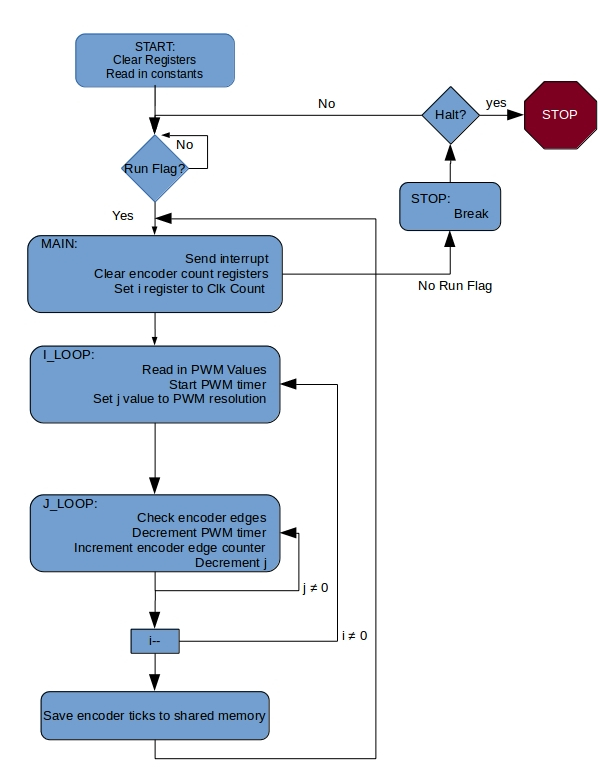
\includegraphics[scale=.7,keepaspectratio=true]{./images_ch3/pru1flow.jpg}
 \caption{Flowchart for PRU 1 Code}
 \label{fig:PRU1_flow}
\end{figure}


\section{PRU 0: PID Controller}

PRU 0 is where the calculation of the PID loop is performed and as such only has to perform calculations every sample period. This may sound like it would be a daunting task but the PID sample period is typically in the 10s of milliseconds. Given that one millisecond equates to 200,000 clock cycles on the PRU, a modest sample period of even 5 milliseconds would result in plenty of time to set and calculate values.  

Because the sampling periods are long (milli-seconds) and the PID code would be a bit daunting to program in assembly, the PRU 0 is coded in C using the PRU Code Generation Tools from Texas Instruments ~\cite{DEREK-MOLLOY}. Not only does this remove the headache of complex assembly code, but also gives the programmer access to functions, structures, and memory pointers. The PRU 0 code is split up between three C files: pru0Lib.c with functions for general PRU0 operation, motorLib.c contains functions for motor control like the PID loop, and pru0.c which holds the main entry point for the program. Along with the C files are header files containing masks and aliases for each library as well as a mem.h file describing the shared memory structure.

\begin{table}

    \begin{tabular}{ | l | p{9cm} |}
    	\hline
	Functions & Description  \\ \hline
	initGPIO(void) & Enables GPIO functionality \\ \hline
	GPIO1pin(int pin, int value) & Controls a GPIO bank 1 pin based on the pin number and value \\ \hline
	GPIO3pin(int pin, int value) & Controls a GPIO bank 3 pin based on the pin number and value \\ \hline
	blinkLED(void) & Toggles the GPIO LED \\ \hline
	enableBuffers(void) & enables the 8 and 4 bit buffers \\ \hline
	disableBuffers(void) & disables the 8 and 4 bit buffers \\ \hline
	initPRU(void) & clears the PRU1 interrupt channel and call initGPIO \\ \hline
	waitForInterrupt(void) & Waits for an interrupt from PRU1 in a while loop. Before leaving it toggles the PRU LED on the board.	 \\ \hline
	killTime(void) & Delays the PRU by roughly 50ms by counting up to 1,000,000. \\ \hline

    \end{tabular}
     \caption{PRU 0 Functions}
 	\label{Tab:PRU0_fun}
\end{table}

Table~\ref{Tab:PRU0_fun} contains a listing of the functions and aliases with descriptions available in pru0Lib.c, pru0Lib.h, pru0.c, and pru0.h. Most of these are concerned with the use of Linux  GPIOs which can be used by PRU0 if desired. One important note is that PRU 0 controls the Linux  GPIO that triggers the on/off status of the buffer chips previously described in Chapter 2 through the two functions enableBuffers() and disableBuffers(). This way the PRU0 acts as the absolute master of the H-bridges and will not enable the motor circuits until entirely set up and ready to begin movement. Most of the PID code and functionality lies within the motorLib.c, motorLib.h and fix.h files and are overviewed in tables~\ref{Tab:PRU0_Motor1} and~\ref{Tab:PRU0_Motor2}.

\begin{table}
    \begin{tabular}{ | l | p{10cm} |}
    	\hline
	Functions & Descriptions  \\ \hline
	FADD(op1, op2) & adds two fixed point numbers. \\ \hline
	FSUB(op1, op2) & subtracts two fixed point numbers. \\ \hline
	FMUL(op1, op2, q) & Mutiplies two fixed point numbers together whose output has a fixed point value of Q. \\ \hline
	FCONV(op1, q1, q2) & Converts op1 from a q1 fixed point to a q2 fixed point. \\ \hline
	haltPRU(void) & Sets the halt flag for PRU1. \\ \hline
	hardBrake(void) & Sets PRU1 up to use the hardbrake. \\ \hline
	cost(void) & Sets PRU1 up to use the soft brake for stopping. \\ \hline
	move(void) & Called when there is a request to move. Main loop of movement control. \\ \hline
\end{tabular}
     \caption{\emph{motorLib} Function and Fix Macros (1 of 2)}
 	\label{Tab:PRU0_Motor1}
\end{table}


\begin{table}
    \begin{tabular}{ | l | p{7cm} |}
    	\hline	
	PID(dc\_motor *motor int32\_t enc) & Called inside move to calculate PID output for each motor, returns the calculated value in a non-fix format \\ \hline
	adjustSetpoint(int32\_t rightVel, int32\_t) & Third PID loop that compares the velocities of the two motor and adjusts their setpoints to drive their difference to zero \\ \hline
	doCommand(command\_code) & State machine that calls functions like move() or haltPRU depending on the command code.	 \\ \hline
	createState(void) & Sets up the state value for PRU1 in shared memory. Sets bits controlling the state of the motors and how they will rotate \\ \hline

    \end{tabular}
     \caption{\emph{motorLib} Function and Fix Macros (2 of 2)}
 	\label{Tab:PRU0_Motor2}
\end{table}

Functions that are part of "motorLib" are accessed through the state machine in the main program which is shown in the flowchart depicted in Figure~\ref{fig:PRU0_flow}. The main program starts by  by calling initPRU(), turning on the buffers, and setting the "mem" pointer equal to the address location of shared memory. Then the main state machine is entered which waits on an exit flag in shared memory and switches state based on the value of command.status in shared memory. 

\begin{sidewaysfigure}[htbp!]
 \centering
 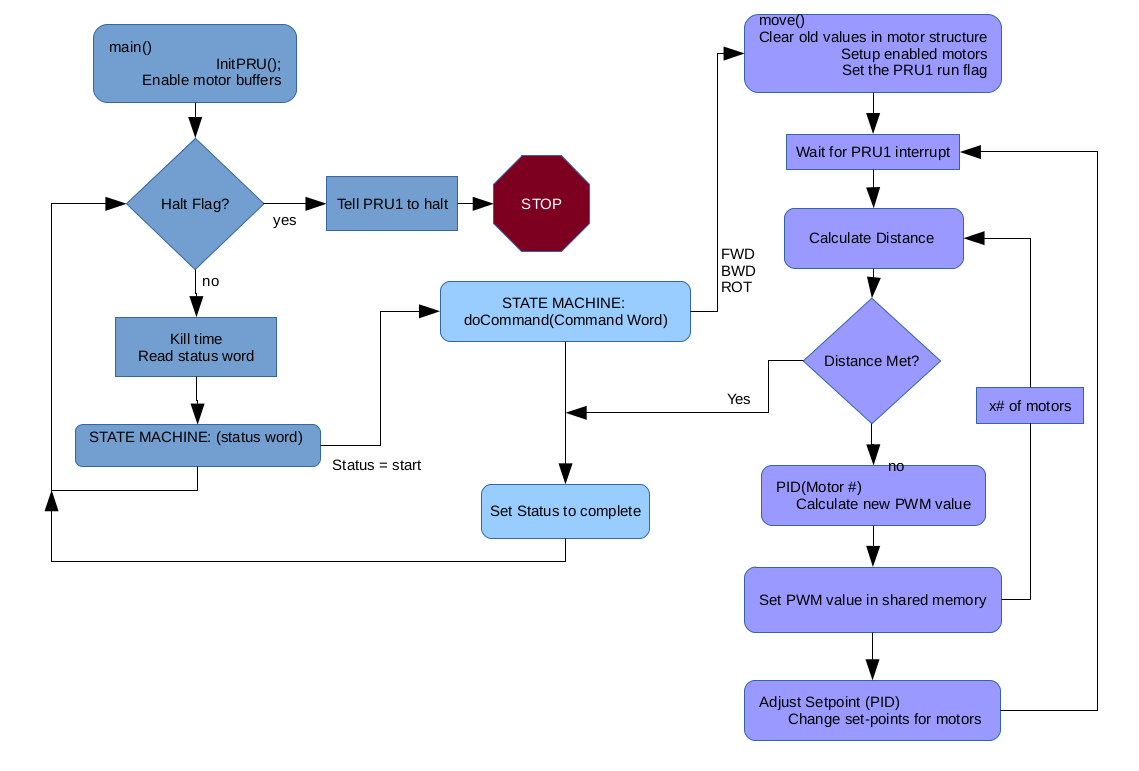
\includegraphics[scale=.5,keepaspectratio=true]{./images_ch3/PRU0FlowNew.png}
 \caption{Code Flowchart of PRU 0 for a Typical Move Command}
 \label{fig:PRU0_flow}
\end{sidewaysfigure}

When PRU 0 sees a START status it calls the doCommand function from motorLib.c, passing the command code also set in shared memory. The doCommand() function is another state machine that will call a function based on the command code sent to it and then set the status to COMPLETED when finished. When following an actual movement command code, like FWD (forward), the move function is called. 

The move function uses values set in shared memory by the ARM core to begin the process of movement. the first order of business is to clear the errors, distance and PWM value for each motor.  The routine createState() is then called to set up each motor for the direction that it needs to spin (clockwise or counterclockwise). After preparations are complete, the run flag is set which causes PRU 1 to start operations and begin the PWM process. From there PRU 0 begins the process of waiting for an interrupt from PRU 1, marking the start of new sample period. When an interrupt is received, PRU 0 begins working on the PID loops for the individual motors. 

First, the total distance traveled by one motor is calculated followed by a check to see if the current set-point need to be increased. Then, if the target distance is not yet reached, work begins on the PID loop for one motor. The PID calculation first starts by saving the previous set-point errors and calculating the new set-point error. From there the delta P, I, and D values are calculated using gain parameters set by the ARM. Before returning the output value it is first checked to see if the output is within the maximum rate of change allowed via the maximum delta cap. Then to make sure that it is within range of the PWM counter another check is ran and capped if needed. 

Returning from the PID calculation, the PWM value is stored in a temporary buffer to be used at the end of the calculation loop. Once each output of the PID controller is calculated the adjustSetpoint() function is called to try and drive the difference in velocities of two motors to zero. This is done in another PID loop and has the same checks on maximum rate of change as the previous one. The output of this PID loop is added to one wheel's set-point and subtracted from the other and which is mirrored by the initial subtracting to find the difference in velocity which is the input into this PID loop. Until the target distance is reached the loop will continue to wait for interrupts from PRU1 recalculating the PID outputs. 

Finally, once the target distance is reached, the run flag for PRU 1 is de-asserted by PR U0 and the program can leave the move function. Returning from the move function back into the doCommand state machine, the status is set to completed and then returns to main. From there, the state machine waits for either a new start status or exit flag. When an exit flag is present a doCommand is called with the parameter HALT\_PRU which will cause PRU 1 to cease operation.  Lastly, the buffers are disabled, the LED is turned off, and an interrupt is sent to the ARM core signaling the end of operation.

\chapter{SIMULATION RESULTS}

\section{Robot Construction}

In this chapter, a demonstration robot will be described in an effort to showcase the power of the SIUE Robot Cape. The robot is simple in design and only has the ability to move around in its environment. It has no additional sensors for interacting with the environment. The goal was to merely to demonstrate the reliable manner in which a robot, using the SIUE Robot cape (and related software), can successfully navigate a typical IEEE robotics arena. 

Along with the robot, the Linux code library will be showcased.  The user libraires which were developed contain routines for movement along with other utilities such as functionality for the I2C devices available on the board. A graphical user interface (GUI) will also be described which was created for ease of use which allow the user to make changes to system parameters. Finally, we conclude the chapter with a description of the program used to evaluate the quality of the work described in this thesis, and we present the results of the standard tests for robot movement.

In order to test the board, the demo robot was constructed using only the BeagleBone Black, the cape, two DC motors with encoders, and batteries. The only functionality that this robot has is the ability to drive forwards, backwards, or rotate. The robot also has a free spinning caster wheel for stability when moving. 

The frame of the robot is created using \emph{Makeblock}\textsuperscript{\textregistered} which is a robotics construction kit aimed at customization and and re-usability. \emph{Makeblock} is the next generation of construction platforms for hobbyist and student oriented robots. \emph{Makeblock} offers strong mechanical parts, mostly made of hardened aluminum.\emph{Makeblock} is the perfect choice to build all kind of robots. Whatever idea a student group might have in mind, it can be implemented using \emph{Makeblock} parts.  The students would simply need to connect the parts together, and the frame of the robot will be constructed in no time at all. \\


\noindent
Features of \emph{Makeblock} include:

\begin{itemize}
\item
high strength aluminum extrusion parts,
\item
smart threaded slot,
\item
high performance timing belt support,
\item
multi-functional adjustable components,
\item
and easy to use, fast to construct.
\end{itemize}

\noindent
Parts available include:
\begin{itemize}
\item
timing belts,
\item
stepper motors,
\item
DC motors with wheel encoders,
\item
linear and rotational bearings,
\item
caster wheels,
\item
sliders, axis and threaded shafts,
\item
and other standard industrial parts.
\end{itemize}

A complete robot can be built from these parts, and \emph{Makeblock} should be considered for use in future competitions. Along with the SIUE Robot Cape, \emph{MakeBlock} offer a total solution to teams competing in the annual IEEE robotics competition. The demonstration robot discussed in the remainder of the chapter is pictured in Figure~\ref{fig:robot_top} and Figure~\ref{fig:robot_bot}. The robot pictured only required a few hours to assemble, is small (approximately 8 inches X 8 inches), light weight, and mechanically sound.  

\begin{figure}[htbp!]
 \centering
 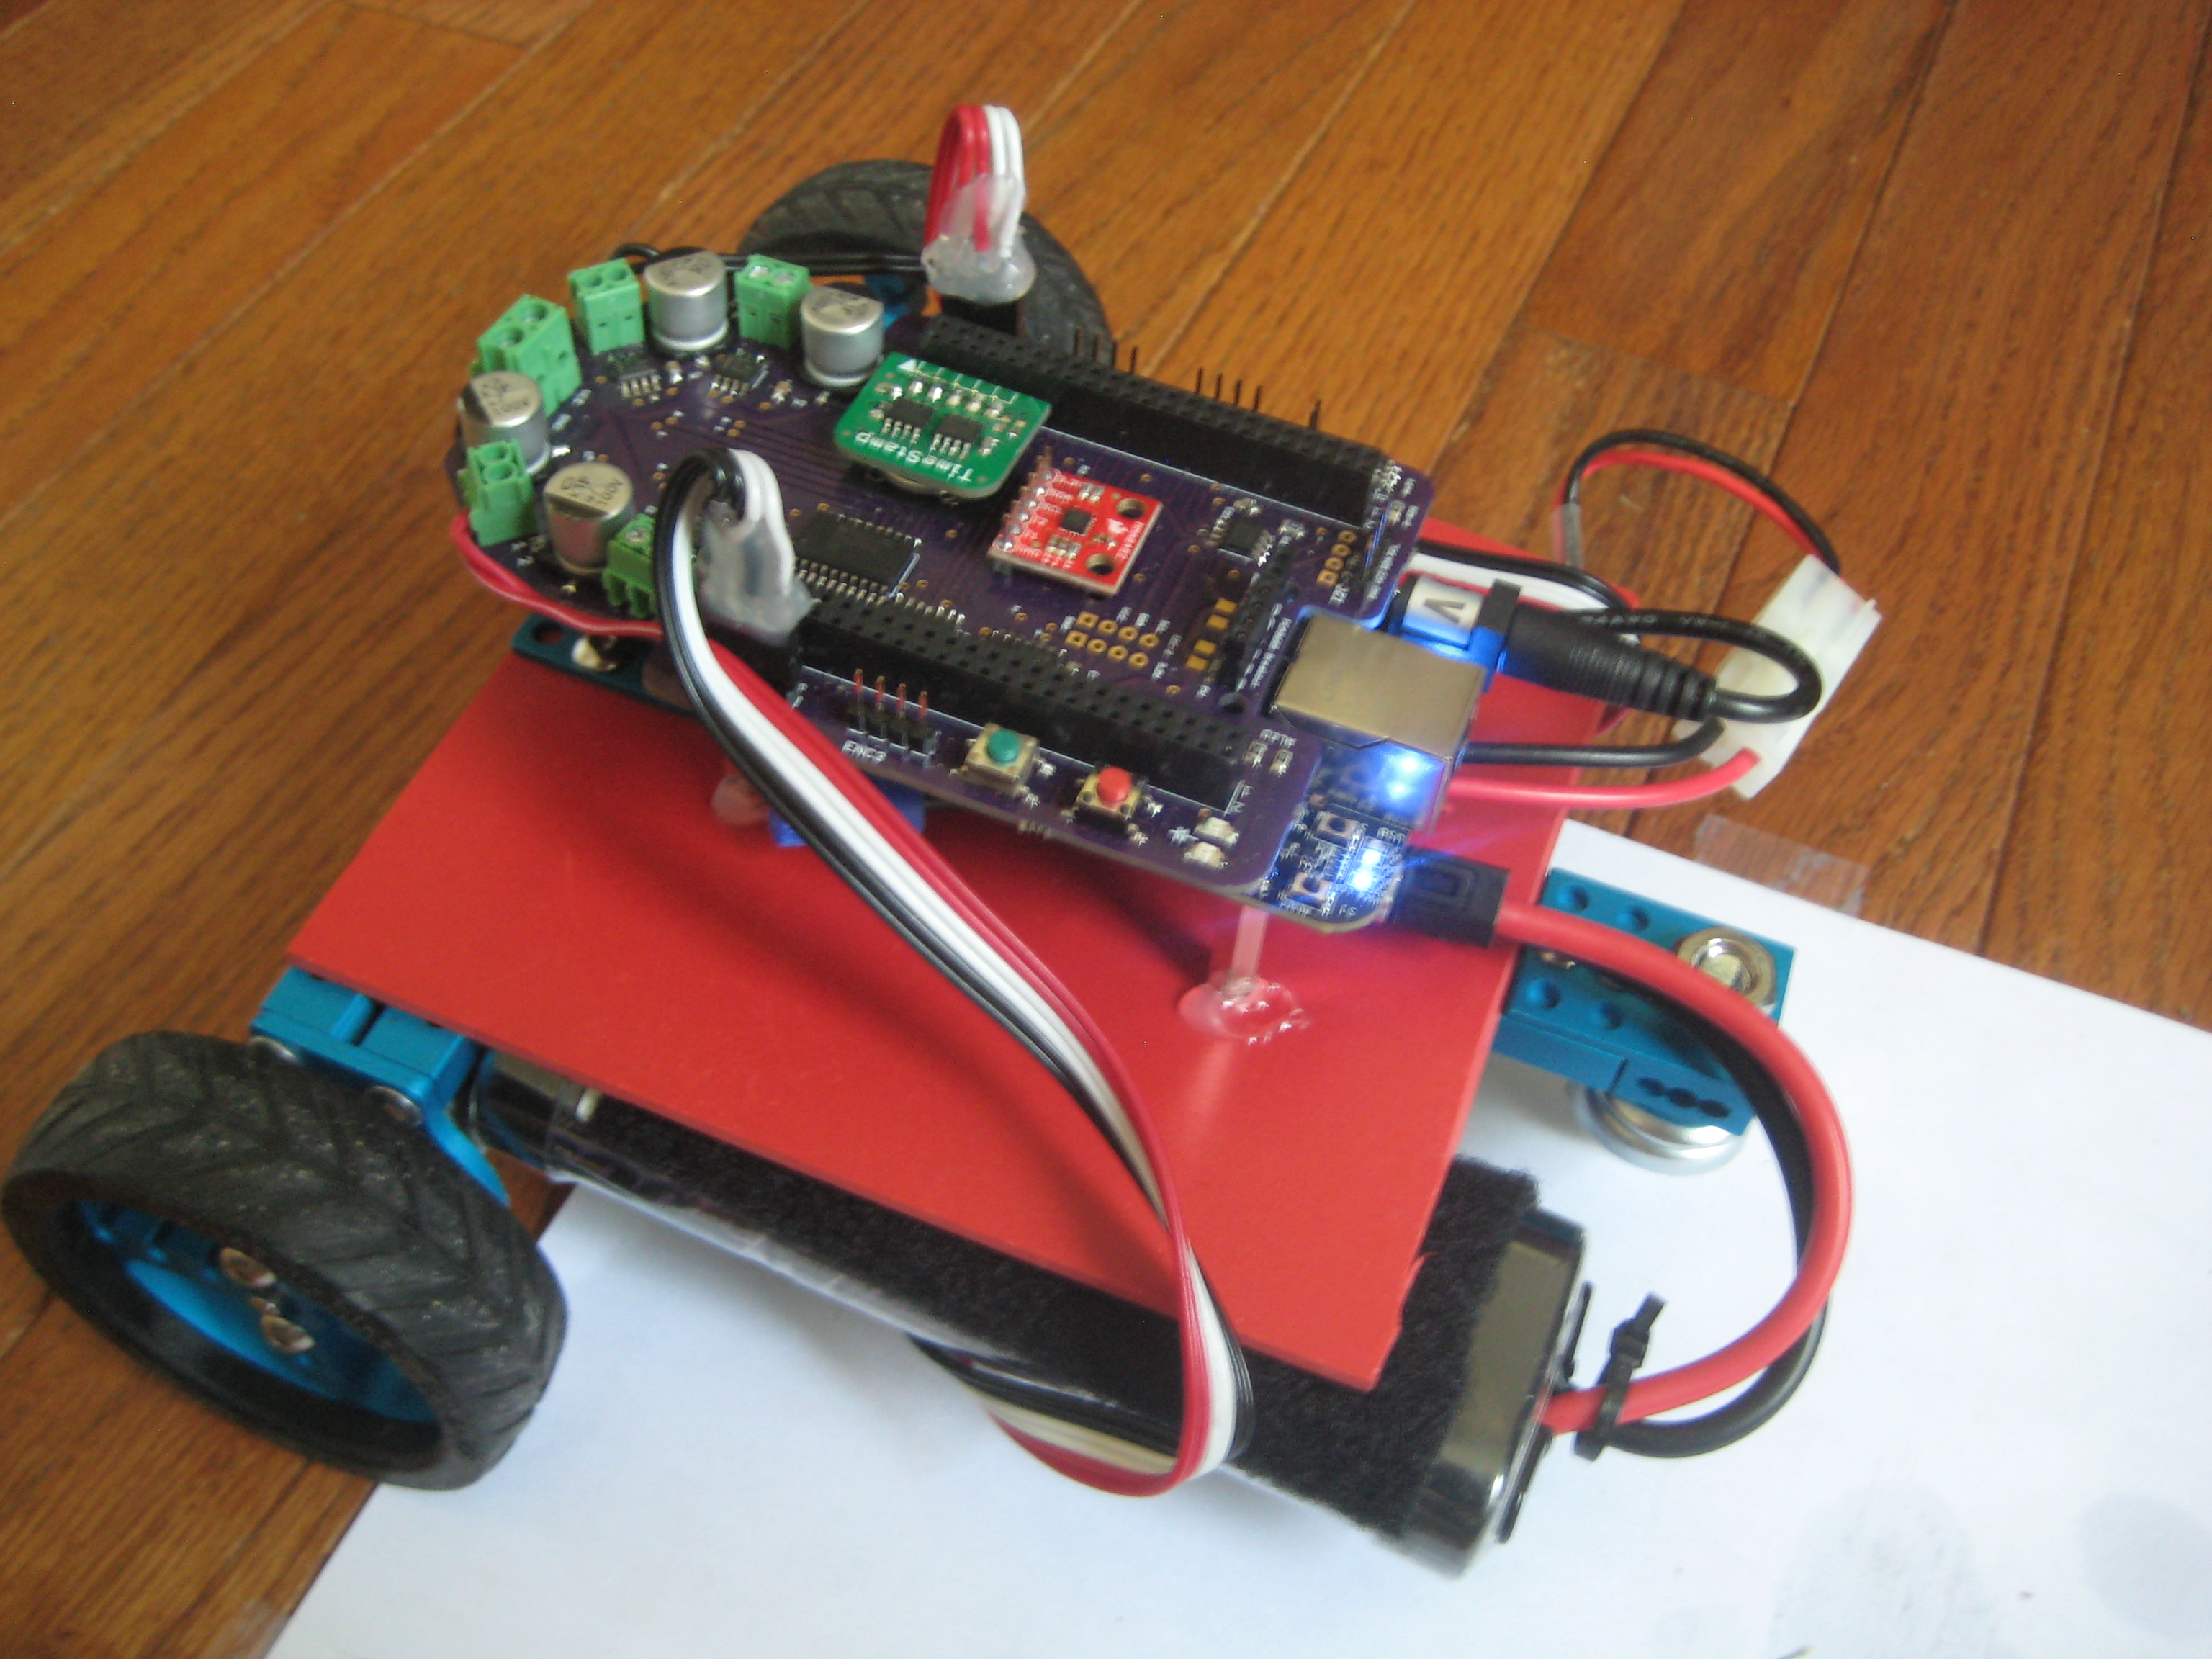
\includegraphics[scale=0.1,keepaspectratio=true]{./images_ch4/robot_top.JPG}
 \caption{Demonstration Robot (top view)}
 \label{fig:robot_top}
\end{figure}

\begin{figure}[htbp!]
 \centering
 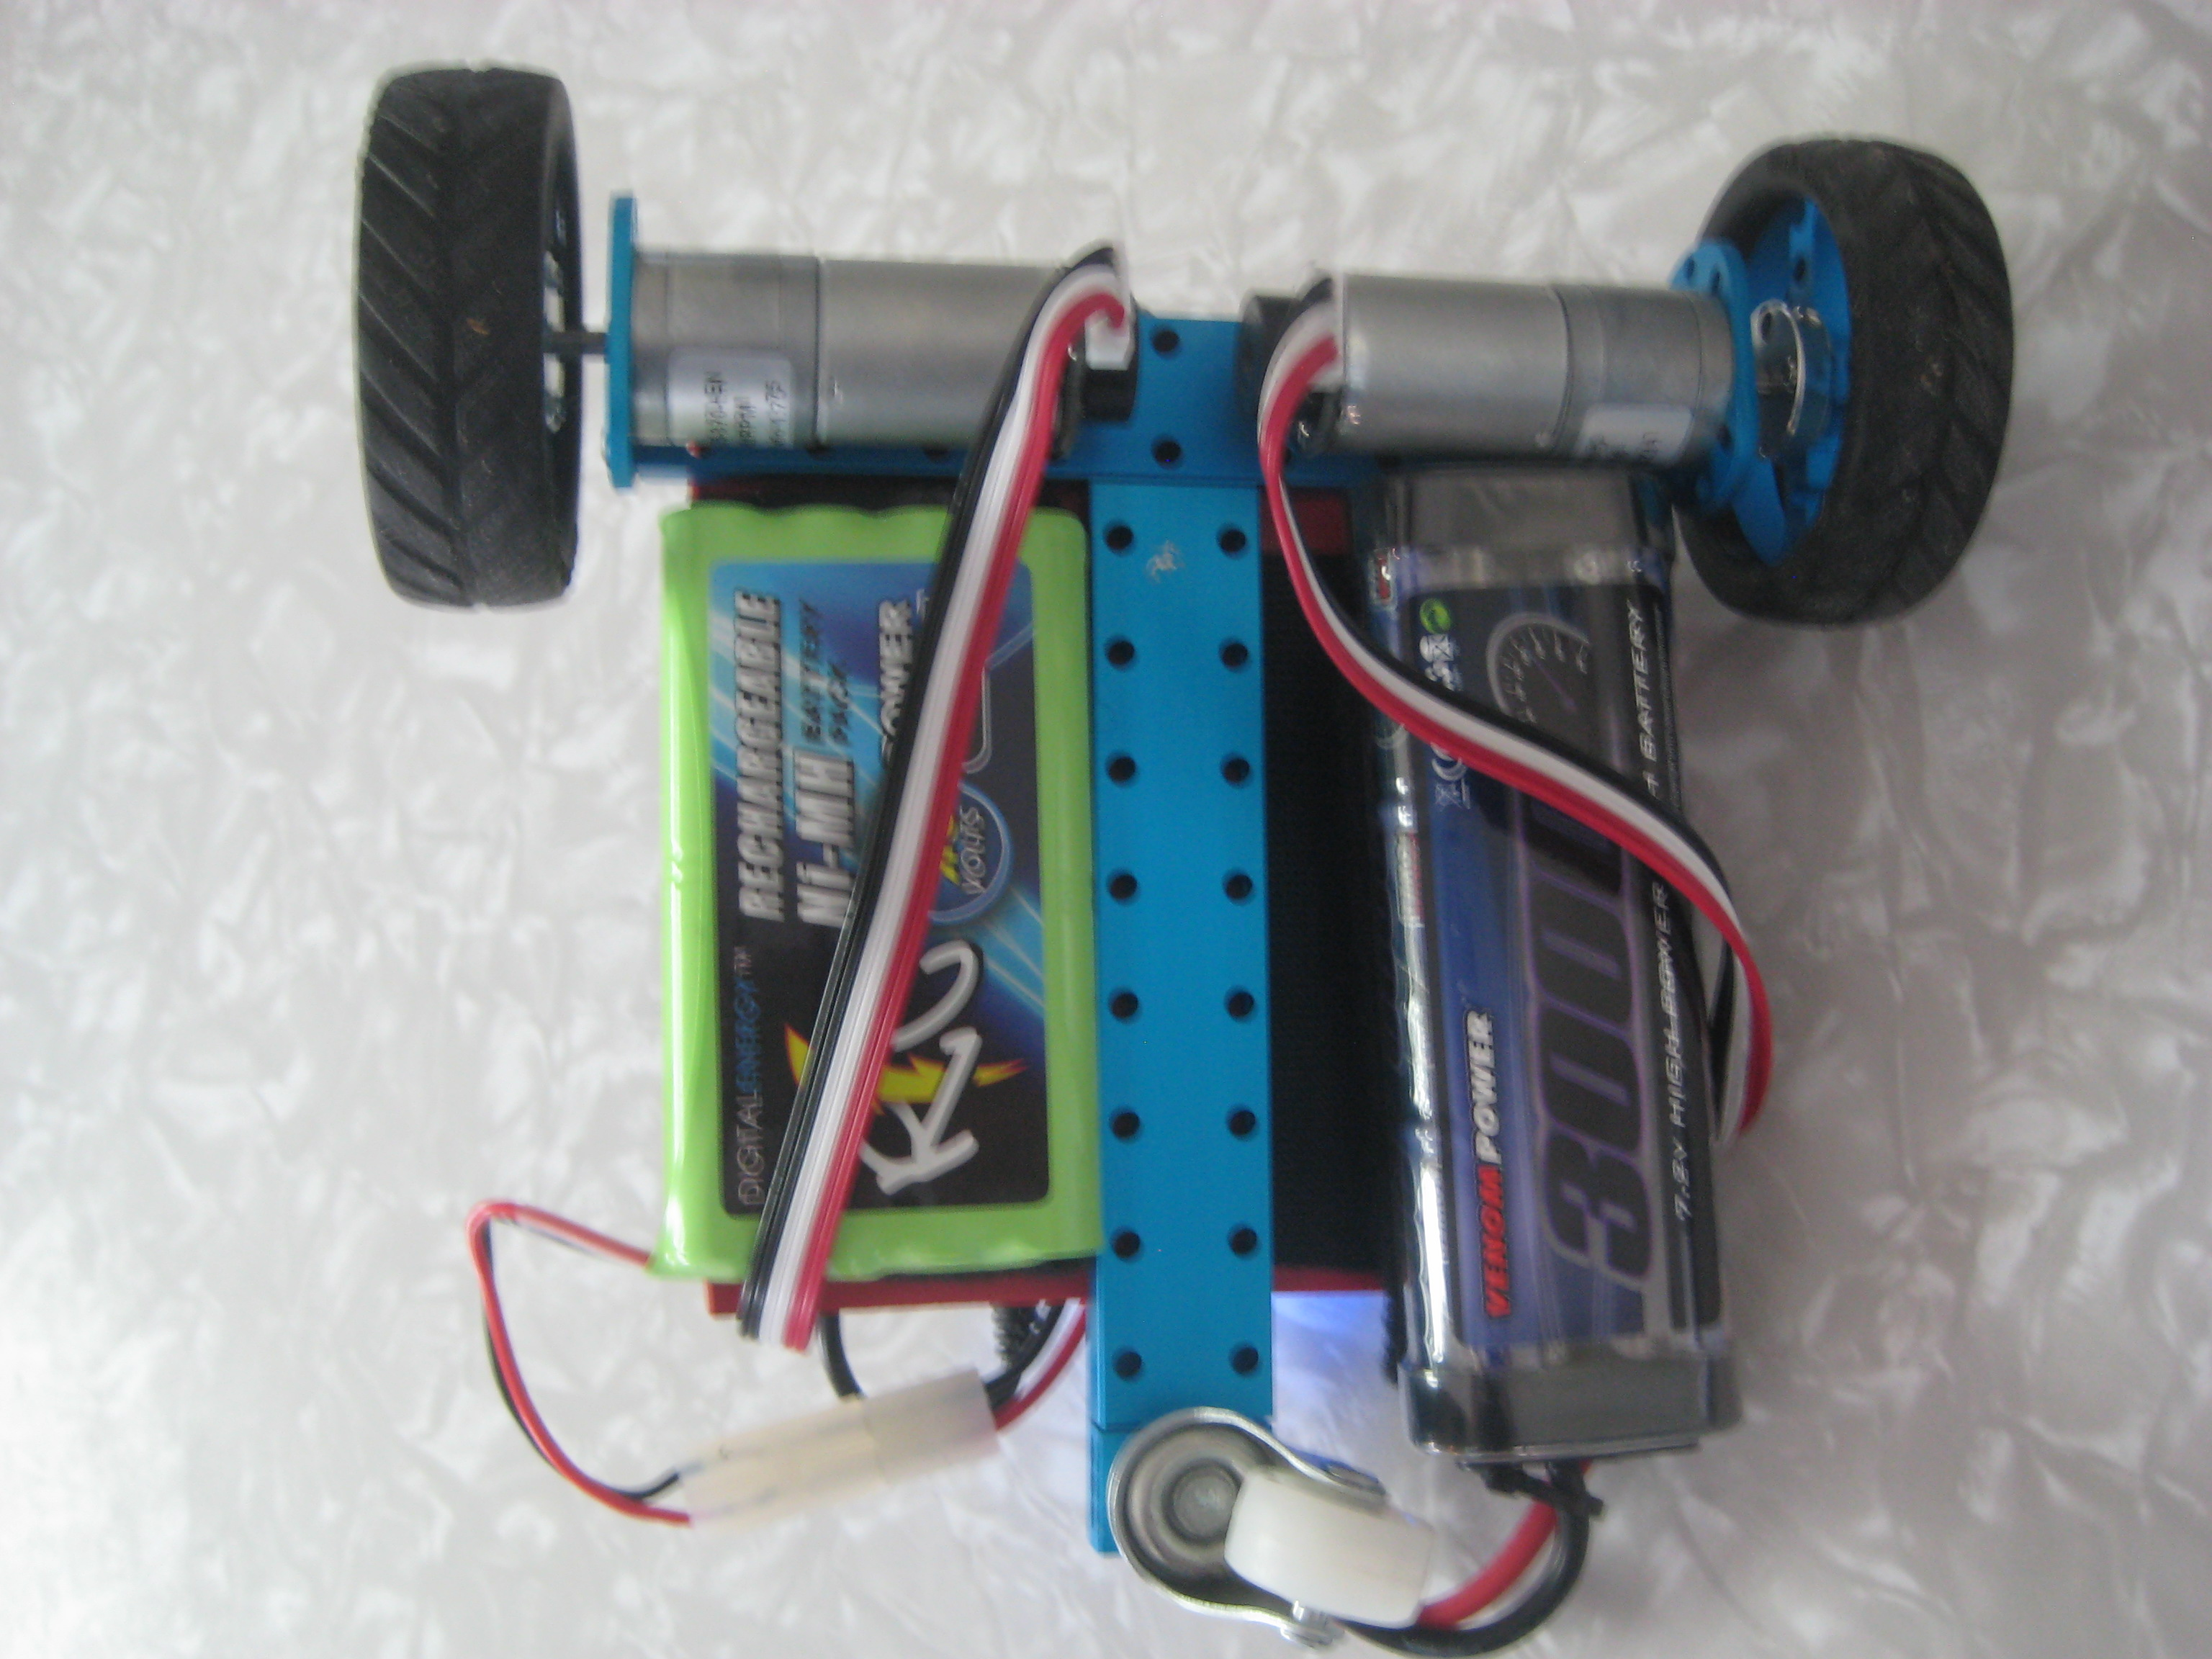
\includegraphics[scale=0.1,keepaspectratio=true]{./images_ch4/robot_bot.JPG}
 \caption{Demonstration Robot (bottom view)}
 \label{fig:robot_bot}
\end{figure}

In the bottom view of the robot two NiMH batteries can be seen.  The 9.6 Volt battery (1600 mA-H) powers the DC motors while the 7.2 Volt battery (3000 mA-H) is converted by a buck converter circuit (located under the BeagleBone Black board and hidden from view) to 5 Volts which is used to power the Black and the SIUE Robot Cape. While not absolutely necessary, the use of two batteries helps ensure that high-frequency noise generated by the PWM circuits does not inadvertently reboot the BeagleBone Black.  This has been a common problem encountered by SIUE robotic teams over the years.

\section{PRU Library Routines}

The Linux code has a collection of functions that are used to access and configure the PRUs using the PRUSSDRV user space library which contains the functionality for basic PRU control, memory mapping and interrupt handling~\cite{PRUWIKI}. Through the PRUSSDRV libary, a user is able to load the PRU with the .bin programing file. The creation of the .bin file needs to be done before executing the main program code on the Linux system. 

One important note is that before the user can call PRUSSDRV functions, the uio\_pruss module needs to be loaded, luckily this is handled by the operating system when a cape (for example, the SIUE Robot Cape) declares use of the PRUs is loaded. The use of the PRUSSDRV is illustrated in Figure~\ref{fig:PRUSS Load} from Derek Molloy's book: Exploring BeagleBone. The figure describes the process of programming the PRUs from the viewpoint of the PRU and the Linux operating system.
 
\begin{figure}[htbp!]
 \centering
 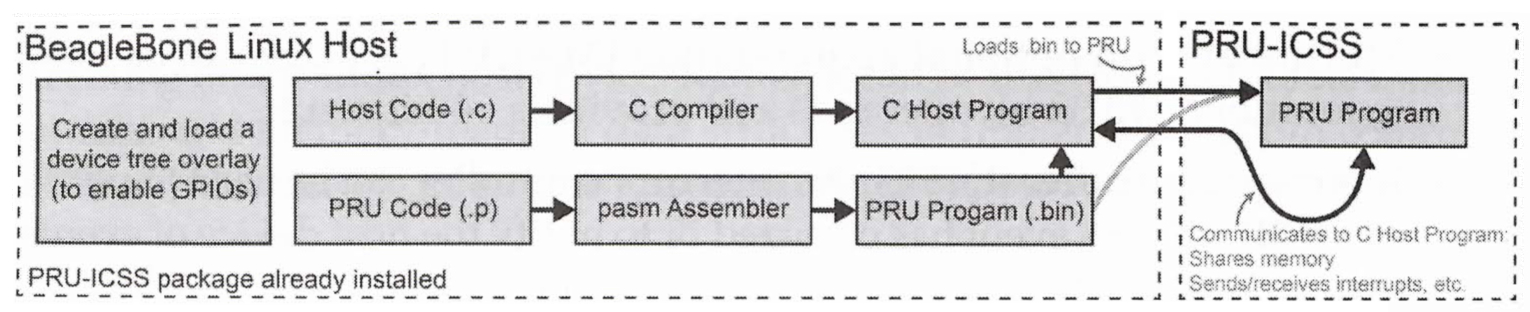
\includegraphics[scale=1.25,keepaspectratio=true]{./images/PRUSSLoad.JPG}
 \caption{Process of Loading and Executing a Program Using PRUSSDRV and Linux}
 \label{fig:PRUSS Load}
\end{figure}

In attempt to simplify this process of calling driver functions, wrappers were created to simplify calls and streamline the process.  These wrappers were bundled together into \emph{PRUlib}. These functions automatically take care of the proper PRU setup for the SIUE Robot Cape by loading in the correct programming files and setting up the correct interrupt channels. The functionality is split between three functions: PRUinit(), PRUstart(), and PRUstop(). PRUinit() handles the setup of the PRUs by calling the initialize function from PRUSSdrv. It also opens the interrupt channels for both PRUs and sets up the shared memory pointer used by the ARM to write values into shared memory. 

It is important to note that PRUinit() relies on global variables declared in the main program which are accessed with extern declarations. PRUstart() handles the loading of the PRU programming files located in the same directory as the executable program. Finally, PRUstop() calls the disable functions for the PRU, halting the PRUs. A listing and description of these functions can be found in Table~\ref{Tab:PRUlibFunctions}. When using  these functions in a program, it is important that PRUinit() and PRUstart() are called before issuing a movement request.

\begin{table}[!htb]
	\centering
    \begin{tabular}{ | l | p{10.5cm}|}
    	\hline
	Functions & Description  \\ \hline
	PRUinit(void) & initializes the PRUs, opens the interrupt channels, and sets up the shared memory pointer (Depends on a global shared\_memory\_t pointer named shared\_memory)  \\ \hline
	PRUstart(void) & Load and execute the binaries for PRUs \\ \hline
	PRUstop(void) &  Disables the PRU and closes the memory mapings for PRUSSdrv\\ \hline
    \end{tabular}
     \caption{\emph{PRUlib} Functions}
 	\label{Tab:PRUlibFunctions}
\end{table}

\section{Beaglebone Black Library Routines}

The BeagleBone Black library or \emph{bbbLib} is a collection of routines created by Gavin Strunk. The library simplifies the job of controlling the various hardware available on the BeagleBone such as the the I2C buses and UART terminals. The use of the library in this thesis is the setup and control of the GPIO pins in the /class/sys/GPIO folder and control of the I2C buses. 

This library can be used by users to create their own drivers for devices that use communication buses such as SPI, UART, or I2C. The ability to access the PWM generators and ADC functionality of the BeagleBone Black is also included in this library but, like any on-board peripheral,they must be set up through the device tree first. Table~\ref{Tab:bbbLibFunctions1} and Table~\ref{Tab:bbbLibFunctions2} describe the \emph{bbbLib} functions that are used by the SIUE Robot Cape library which will be described in the next section of this thesis. 

\begin{table}[!htb]
	\centering
    \begin{tabular}{ | p{7cm} | p{8cm}|}
    	\hline
	Functions & Description  \\ \hline
	initPin(int pinnum) & Initializes a GPIO pin with a corresponding GPIO number \\ \hline
	setPinDirection(int pinnum, char* dir) & Sets the GPIO pin direction (input or output) based on the GPIO number and the direction specified. Inputs need to be setup as receivers in the device tree overlay. \\ \hline
	setPinValue(int pinnum, int value) &  Sets the output pin value to a logic high or low\\ \hline
	getPinValue(int pinnum) & Returns the logic level value of the input pin\\ \hline
	i2c\_open(unsigned char bus, unsigned char addr) & Returns a handle to access a I2C device given a bus and an address\\ \hline
	i2c\_write(int handle, unsiged char* buf, unsiged char length) & Puts a char buffer of size length given the I2C handle\\ \hline
	i2c\_write\_read(int handle, unsigned char addr\_w, unsigned char *buf\_w, unsigned int len\_w, unsigned char addr\_r, unsigned char *buf\_r, unsigned int len\_r) & Preforms a write/read operation on the I2C bus given the handle (necessary for reading from the I2C device as a write from the master telling the device what to send before the device controls the bus) \\ \hline
	i2c\_close(int handle) & Closes the I2C handle\\ \hline    
    \end{tabular}
     \caption{\emph{bbbLib} Functions (1 of 2) }
 	\label{Tab:bbbLibFunctions1}
\end{table}

\begin{table}[!htb]
	\centering
	\begin{tabular}{|l|p{8cm}|}
		\hline
		Functions & Description \\ \hline
		pauseSec(int sec) & Halts the program execution for a set number of seconds \\ \hline
		delay\_ms(unsigned int msec) & halts the program execution for a set number of microseconds \\ \hline
		pauseNanoSec(long nano) & Halts the program execution for a set number of nanoseconds \\ \hline
	\end{tabular}
    \caption{\emph{bbbLib} Functions (2 of 2) }
 	\label{Tab:bbbLibFunctions2}
\end{table}

\section{Robot Library Routines}

A series of routines were developed to support the SIUE Robot Cape.  These routines where bundled together into what we will call \emph{robotLib}. This library handles the setup of the environment that will be used to control the motors by placing values into shared memory. As already mentioned, the shared memory is used by all three processors (ARM, PRU 0, PRU 1) to share information and to communicate with one another. The collection of functions that are available in \emph{robotLib} are listed in Table~\ref{Tab:robotLibFun1}, Table~\ref{Tab:robotLibFun2}, and Table~\ref{Tab:robotLibFun3}. 

In Table~\ref{Tab:robotLibFun1} the first four functions are used for initialization related to memory and GPIO. These functions use a configuration string to setup variables used by the motor controller. The string is either read from a file (robot.config) or obtained from the GUI (Graphical User Interface) described in the next section. Using this configuration information the configPRU(), updateMotor(), and initSetpointPID() routines deal with actual loading of values into shared memory.  

In many cases floating-point numbers are first converted to fixed-point before the values are stored in shared memory. The PRUs use encoder "tics" as a distance measure.  Routines were created to convert from inches-to-tics and from tics-to-inches. Query functions are used to extract the motor and command status from shared memory and are also used in the waitForIdle() and waitrForComplete() functions.

Table~\ref{Tab:robotLibFun3} summarizes functions related to movement. Functions like fwd(), bwd(), rotate(), left() and right() call updateMotor() to initialize the DC motor structures and then eventually request movement by changing the command status value saved in shared memory.  Figure~\ref{fig:ARMFlow} diagrams the sequence of events initiated by a fwd() call. 

\begin{sidewaysfigure}[htbp!]
	\centering
	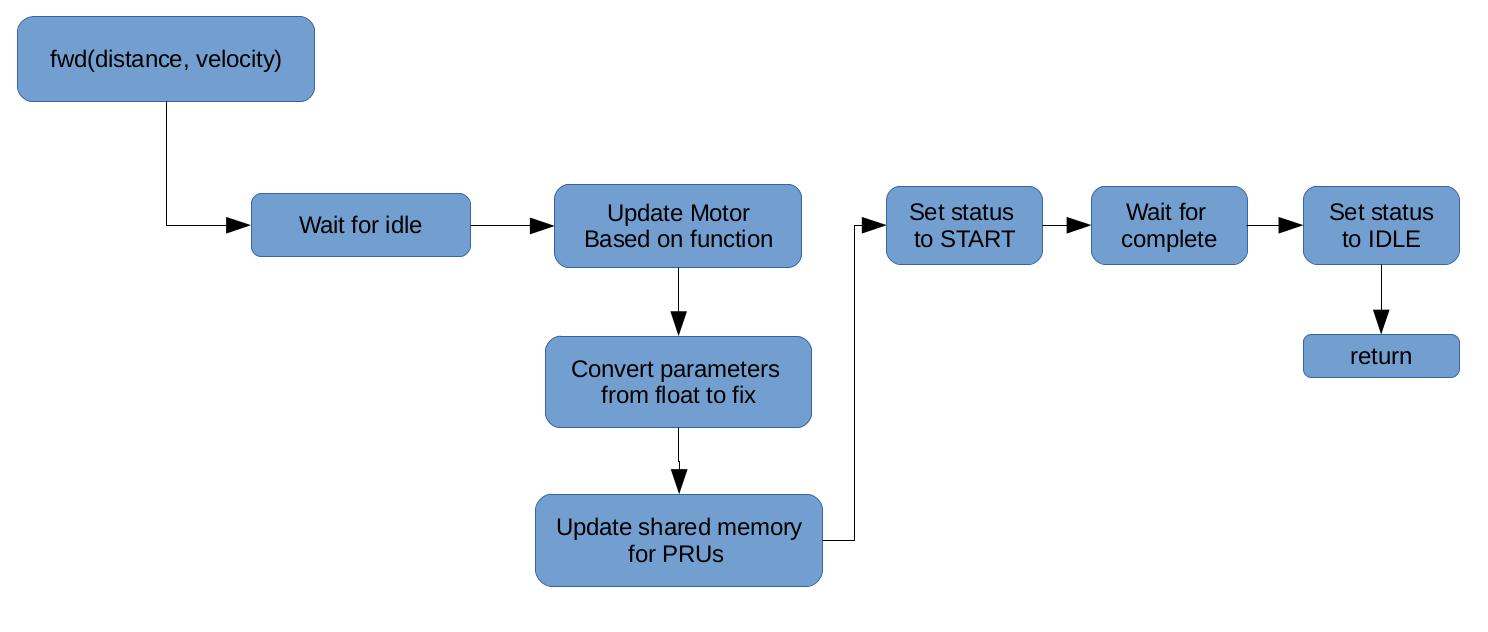
\includegraphics[scale=.4]{./images/ArmFlow.png}
	\caption{ARM fwd() Routine Flow Diagram}
	\label{fig:ARMFlow}
\end{sidewaysfigure}

When fwd() is called, it checks to make sure that the motor is in an "idle" state. Following the check, it calls the updateMotor() routine which performs the necessary conversions from the requested operation in inches to tics as well as converts numbers from a floating-point to fixed-point format before storing these values into shared memory. After setup for movement is complete the status is set to "start" to notify the PRU to start motor operation given the current parameters. 

The ARM core then waits for a complete calling waitForComplete and then sets the status to idle denoting that it is done with its operation. The rest of the movement commands follow a very similar flow with the rotate requiring a degree of rotation instead of the travel distance. These functions are all that is required for users to get a constructed robot moving after calling the appropriate setup functions providing ease of use to the user. 

		
\begin{table}[htbp!]
	\centering
	\begin{tabular}{|l|p{8cm}|}
		\hline
		Functions & Description \\ \hline
		GPIOinit(void) & Sets up the necessary GPIO pins such as the user LEDs and buffer enable pin \\ \hline
		getGUIvars(char *str) & Uses sscanf to read the string outputted by the GUI environment to setup the values in the GUIvars structure which holds constants for the motor controller operation. \\ \hline
		loadGuiVarsFromFile(char *str) & Opens a configuration file to setup the GUIvars structure. \\ \hline
		configPRU(void) & Configures the PRUs, specificity the shared memory, with the values from GUIvars preforming necessary conversions in the process \\ \hline
		initSetpointPID(void) & Setup shared memory with the values for the setpoint PID loop. Called in configPRU \\ \hline
		resetPRU(void) & Sets the master PRU in a IDLE state \\ \hline
		waitForIdle(void) & Waits until an IDLE state is set in shared memory by the master PRU \\ \hline
		waitForComplete(void) & Waits until a COMPLETE state is set in memory by the master PRU \\ \hline
		
		\end{tabular}
		 \caption{\emph{robotLib} Functions (1 of 3)}
 	\label{Tab:robotLibFun1}
\end{table} 
		
\begin{table}[htbp!]
	\centering
	\begin{tabular}{|p{6cm} | p{9cm}|}
		\hline
		Functions & Description \\ \hline
		inches2tics(float inches) & Returns a fixed point conversion of inches to inches based on shared memory values \\ \hline
		tics2inches(int32\_t tics) & Returns a float conversion of ticks to inches based on shared memory values \\ \hline 
		updateMotor(int motor\_num, int dir, int brakeType, float distance, float velocity) & Updates the corresponding DC\_motor\_t structure in shared memory with the parameters for a movement operation. Performs the necessary conversions before updating the structure. This is called by the fwd, bwd, left, right, and rotate functions. \\ \hline
		queryMotor(int motor\_num, int item) & Returns the designated item from the designated DC\_motor\_t structure in shared memory (set-point, wheel direction, target distance, etc.) \\ \hline
		query(int item) & Returns the designated item from shared memory, only for current command or status. \\ \hline
		turnLED(int state) & Sets the GPIO LED on board based on the state. \\ \hline
		buttonPress(void)  & Returns the current value of the GPIO button. \\ \hline
		memoryDump(void) & Prints values in shared memory to a text file in the execution directory. \\ \hline
		
		\end{tabular}
		 \caption{\emph{robotLib} Functions (2 of 3)}
 	\label{Tab:robotLibFun2}
\end{table}
				
\begin{table}[htbp!]
	\centering
	\begin{tabular}{|p{6cm} | p{9cm}|}
		\hline
		Functions & Description \\ \hline
		fwd(float distance, float velocity) & Requests a forward movement operation from the motor controller given the parameters. (velocity in inches per second) \\ \hline
		bwd(float distance, float velocity) & Requests a backward movement operation from the motor controller given the parameters. (velocity in inches per second) \\ \hline
		rotate(float degrees, float velocity, int direction) & Requests a rotation operation from the motor controller given the  parameters. Rotates up to 360$^{\circ}$ in a clockwise or counter clockwise fashion.  \\ \hline
		left(void) & Calls rotate to turn the robot 90 degrees in a counter clockwise direction at 6" per second. \\ \hline
		right(void) & Calls rotate to turn the robot 90 degrees in a clockwise direction at 6" per second. \\ \hline
		applyBrake(void) & Requests a hard brake from the motor controller. \\ \hline
		
		\end{tabular}
		 \caption{\emph{robotLib} Functions (3 of 3)}
 	\label{Tab:robotLibFun3}
\end{table}


\section{Graphical User Interface}

The GUI (Graphical User Interface) for this application was created using Tcl/Tk (Tool Command Language with GUI Tool Kit). The GUI serves as system configuration interface. A Tcl shell is launched from main (\emph{i.e.} beaglebot.c) and a two-way pipe in started. The two-way pipe allows the C code to communicate with the Tcl shell by simply reading from "stdin" and writing to "stdout".  A command is sent to the Tcl shel to source the "gui.tcl" file. The configuration data is returned (via "stdin") to the C calling routine as a string.  The parameters are colon delimited.

The advantage to the above approach is that the GUI can be debugged using a standard Tcl shell (on any platform that supports Tcl/Tk) and support for Tcl/Tk is readily available. The GUI Toolkit (Tk) makes the creation of a GUI a relatively simple and painless matter. Furthermore, the use of Tcl/Tk makes is easy for future SIUE teams to quickly and easily modify the GUI as the the need to do so arises. The colon-delimited string returned to the C calling routine is easily parsed. The paramters are stored in a global C structure called GUIvars.

The GUI screen is displayed in Figure~\ref{fig:GUI}. It contains a series of sliders, text boxes, and check boxes.  The user can select which I2C peripherals (servos, sonars, accelerometer, real-time clock) are required. This is important since trying to access a non-existent device on an I2C bus will cause the ARM processor to hang. It is also important that the user select the motor type: stepper or DC.  As described in earlier chapters, the hardware on the SIUE Robot Cape can support either 2 stepper or (up to) 4 DC motors. After selecting the motor type, it is important that the user enable the appropriate motor drivers. (The names used by the GUI correspond to the names silkscreened on the PCB).

\begin{figure}[!htbp]
 \centering
 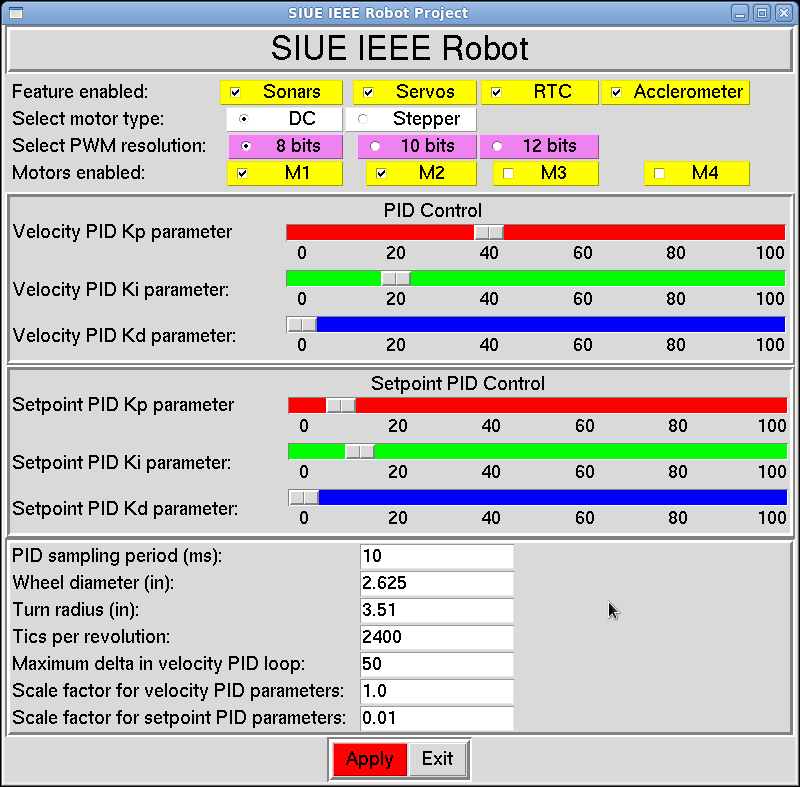
\includegraphics[scale=.5,keepaspectratio=true]{./images/GUI.png}
 \caption{Tcl/Tk GUI Ensures Ease-Of-Use}
 \label{fig:GUI}
\end{figure}

While the user can select PWM resolution (8, 10, or 12 bits), testing revealed that the 8-bit mode should be used. Robot movement was \textbf{not} improved with 10 or 12 bit resolution and use of the other modes resulted in an audible tone when the motors were running. The author suggests that the PWM resolution be removed from the GUI at some point in the future.

There are sliders for the PID gains which are multiplied by scale factors that can also be specified. The PID control sliders set the gain factors for the motor velocity PID loops. The \emph{setpoint} PID sliders are used in the master PID loop that implments the differential velocity control.  Lastly, there are text boxes so the user can change parameters like sampling period, wheel diameter, tics per revolution, turn radius, \emph{etc}. 

One important value that can be changed is the maximum "delta" used by the PID loops.  Recall, the differential form of the PID algortion was used in this work, where the next PWM output is determined by taking the current value and adding a "delta".  By being able to control the maximum "delta", we one prevent wheel slippage (by effectively limiting acceleration), and one can also help improve loop stability.  Emperical evidence suggests that $K_d$ can usually be set to zero in most mobile robot applications.  

When all parameters are set, hitting the apply button will send the configuration string to "stdout". The string is parsed and the configuration data is stored in the global structure, GUIvars. This configuration data can then be accessed by the various routines in \emph{robotLib}. The "Apply" button in the GUI turns from red to green in color when it is pressed. 

\section{Demonstration Program}

The demonstration program (beaglebot.c) was created to demonstrate the movement capabilities of the board. As mentioned earlier, there is no environmental feedback for the demo robot other than encoder feedback so the only action it can really perform is driving which is exactly what it does!  The demonstration program executes the following movements.

\begin{enumerate}
\item
Drive forward for 48 inches at a speed of 12 inches per second.
\item
Make a left turn and then forward at 12 inches per second for a distance of 24 inches.
\item
Make a left turn and then forward at 12 inches per second fot a distance of 48 inches.
\item
Make a left turn and then forward at 12 inches per second for a distance of 24 inches.
\item
Pivot counter-clockwise 180$^{\circ}$ and traverse the path desribed above in reverse direction, making right turns, and then returning to orginal position.
\item
Drive forward again at the same rate and perform another 180$^{\circ}$ turn.
\item
This process repeats twice and then the robot stops in "precisely" the same spot and orientation from which it started,
\end{enumerate}

All turns and pivots where executes at a speed of 6 inches per second.  The slower speed on turns greatly improved reliability. The quality of the movements was judged on how "precisely" the robot returned to the starting position.  In many of the mobile robot contests that our teams have participated in over the years, the robot must start at a prescribed location in the arena, navigate to other locations in the arena, and then return to the original starting location.  The demonstration program was intended to replicate the type of movement that might be expected of the robot in future competitions.

\section{Results of Navigation Test}

When running the demo program the robot travels a total of 32 feet or a little over 10.6 yards before returning to its original starting position. The robot begins on a sheet of paper to mark its starting point and ends on the same piece of paper. This test attempts to demonstrate the accuracy of the motor controller over long distances of movement where the systematic and non-systematic errors of robot movement would accumulate and could be easily visible. 

In the trial runs, the robot perforned extremely well and returned to the sheet of paper each time with slight variation in its stopping position. The restults of two test runs can be seen in Figure~\ref{fig:robottest1} and Figure~\ref{fig:robottest2}.  While this is not a standardized test (they usually involve driving 12 feet rather than 4 feet as we did), the test is in the same spirit as the standardized test.  The use of shorter distances is justified because it is consistent with movement required in the mobile robot arenas (typically just 8 feet x 8 feet) that our teams compete in.

\newpage
\begin{figure}[!t]
 \centering
 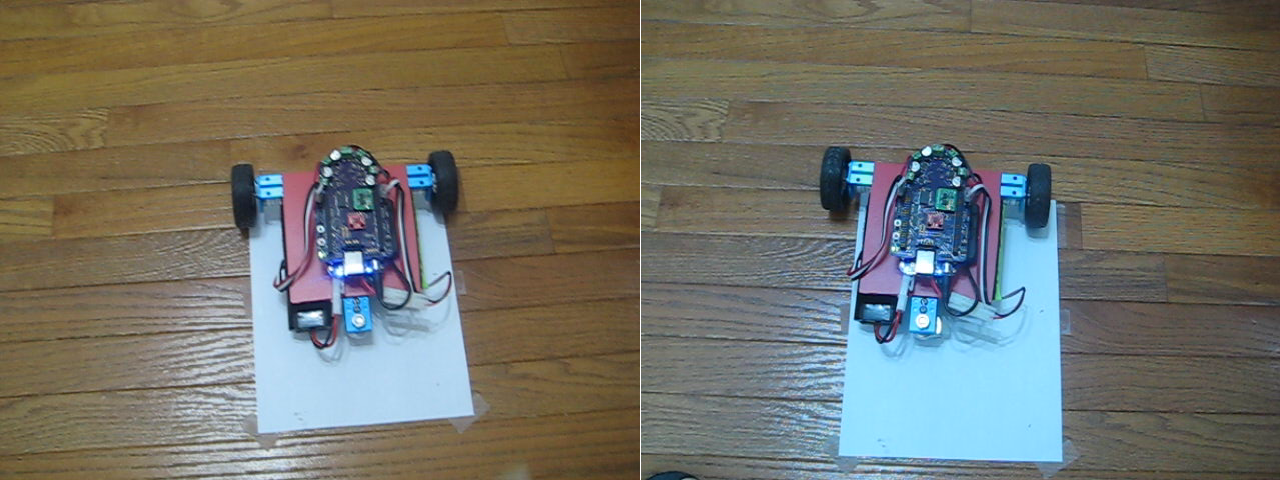
\includegraphics[scale=.35,keepaspectratio=true]{./images/robot-test1.png}
 \caption{Robot Before (left) and After (right) Run - Trial \#1}
 \label{fig:robottest1}
\end{figure}

\begin{figure}[!t]
 \centering
 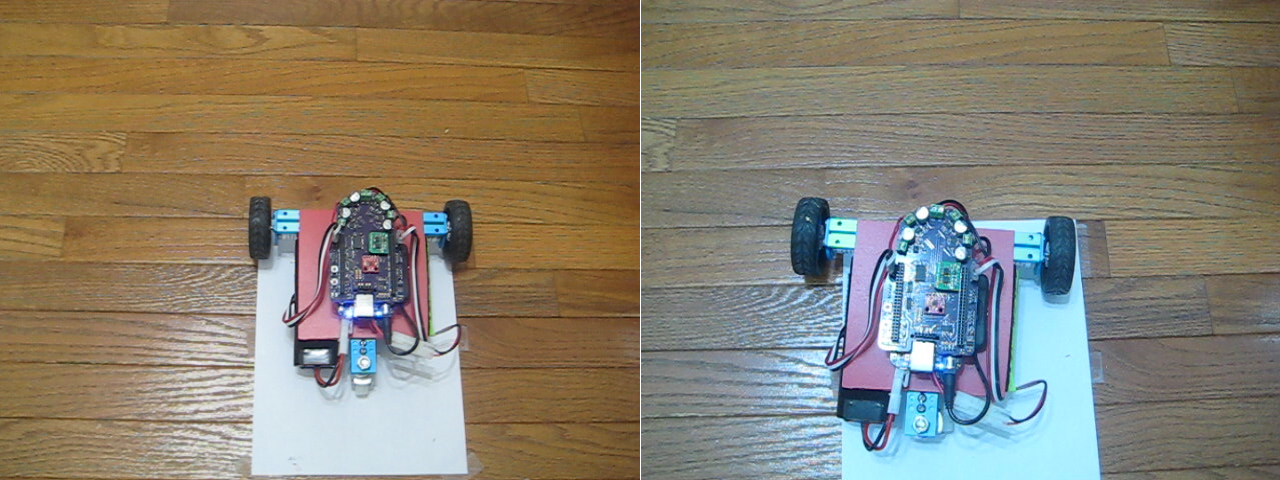
\includegraphics[scale=.35,keepaspectratio=true]{./images/robot-test2.png}
 \caption{Robot before (left) and after (right) After Run, - Trial \#2}
 \label{fig:robottest2}
\end{figure}


\chapter{SUMMARY, COMCLUSIONS, AND FUTURE WORK}

\section{Summary}

Using the Texas Instruments' BeagleBone Black, a custom board (the SIUE Robot Cape), and \emph{Makeblock}\textsuperscript{\textregistered} (mechanical parts), a small, easy-to-use, yet powerful robotics platform has been developed and the its usefulness has been demonstrated in this thesis. The platform which has been described in detail supports either four DC motors with quadrature wheel encoders or two stepper motors running open-loop. The ability to independently control four DC motors with encoder feedback affords the user the option of employing four omni-directional wheels in the robot design.

In addition to providing reliable movement, the SIUE Robot Cape supports two user I2C buses for quickly and easily accessing a wide variety of peripherals, a real-time clock, a 16-channel servo motor controller, and an accelerometer. The system can be powered from standard RC car NiMH batteries.  The overall system strikes the right balance between flexibility and ease-of-use. In the pursuit of this end, a graphical user interface was developed to allow users to quickly configure the system and tune the various PID loops used for guaranteeing reliable navigation. 

\section{Conclusions}

A large amount of work went into making the cape as easy to use as possible and also into making the platform suitable for use by SIUE student robotic groups in the future. Now that this platform is available, students and hobbyists may use the board in a number of different ways and applications. The cape is highly integrated with Texas Instruments' BeagleBone Black single-board computer, and the software described in this thesis can be easily changed to suit a myriad of mobile robot applications. 

The PRUs do an excellent job of handling PID calculation, PWM signal generation, and reading of encoder feedback without taxing the main ARM system. The circuit board cape has a large amount of built in functionality and can be expanded by stacking capes or using other user circuit boards. With a two wheel differential drive design, the cape and related software desribed in this thesis performed well. The test robot produced a small amount of noticeable drift but with additional feedback (from the accelerometer), it could be made to be even more precise in its movements. Hopefully the SIUE Robot Cape will be useful for years to come.  In short, the design objectives put forth in Chapter 1 have been succesively met.

\section{Future Work}

Much more work can be done to refine and improve the SIUE Robot Cape. Currently, only about half of the full functionality envisioned by the author at the onset of this project is available to the user. The following is list of possible improvements and work which still needs to be done in order to unlock the full potential of this cape.
\begin{itemize}
\item 
Add utilities for mecanum (omni-directional) wheel support, using all four motor drivers. At present, only two-wheel operation is fully supported by the software.
\item
Add support for arbitrary movement. In the current implementation only straight-line moves and pivots are supported.
\item 
Add functionality for stepper motor use and control.
\item
 Add the ability to make the the movement operations non-blocking. At present, control is not returned to the calling routine until the movement commands completes.  While at times this is desirable, one can conceive of cases where it would be desirable to move on to another task while the move command is being executed.  Because command status is stored in shared memory, the monitoring of whether the move command is complete or not could be left to another routine.  
\item
Add support for threads.  It is well-known that multi-threading is quite useful in robotic applications.
\item 
Add RTC functionality for updating the system clock.  Moreover, while the RTC was tested, at present no support for it is included in the current implementation of \emph{robotLib}.
\item 
Implement a better movement tracking sensor, one that not only measures acceleration readings but, through a digital gyroscope, angular velocity as well.
\item 
Update to the 4.1 Kernal for use with the BeagleBone Green.
\item 
Turn existing "libraries" into true C dynamically linkable libraries.
\end{itemize}

This is just a partial list, and the author is confident that future users of the cape and its software will only be limited by their own imaginations.  It is the author's sincere hope that the work reported on in this thesis will spur future SIUE IEEE robotic teams to achieve great results in future competitions.

\references %single spacing / arabic numeral paginations, adds "REFERENCES" to table of contents

%%%% for bibtex

%If you want to use bibtex  use the following lines, where your .bib file is called 'yourbib.bib'

\bibliographystyle{apalike}
\bibliography{./cfaber_thesis}

% If you have only a single appendix, do it this way.

\multipleappendices
\lstset{
         language=C,
         basicstyle=\scriptsize\ttfamily,
         emptylines=0, 
         lineskip=1pt,
         %numbers=left,            
         numberstyle=\tiny,         
         stepnumber=2,              
         numbersep=5pt,             
         tabsize=3,                
         extendedchars=true,       
         breaklines=true,            
         commentstyle=\color{blue},
         keywordstyle=\color{red},
            frame=b,         
 %        keywordstyle=[1]\textbf,    
 %        keywordstyle=[2]\textbf,    
 %        keywordstyle=[3]\textbf,  
 %        keywordstyle=[4]\textbf,   \
         stringstyle=\scriptsize\color{green}\ttfamily, 
         showspaces=false,         
         showtabs=false,            
%         xleftmargin=17pt,
%         framexleftmargin=17pt,
%         framexrightmargin=5pt,
%         framexbottommargin=4pt,
         %backgroundcolor=\color{lightgray},
         showstringspaces=false           
 }

\chapter{Global Defines and Structures}
\lstinputlisting{./include/mem.h}

\chapter{Fixed-point Macros}
\lstinputlisting{./include/fix.h}

\chapter{PRU 1 Assembly Code}

\section{pru1.h}
\lstinputlisting{./pru_code/pru1.h}
\newpage
\section{pru1.p}
\lstinputlisting{./pru_code/pru1.p}

\chapter{PRU 0 C Code}

\section{pru0.h}
\lstinputlisting{./pru_code/pru0.h}
\newpage
\section{pru0.c}
\lstinputlisting{./pru_code/pru0.c}
\newpage
\section{pru0Lib.h}
\lstinputlisting{./pru_code/pru0Lib.h}
\newpage
\section{pru0Lib.c}
\lstinputlisting{./pru_code/pru0Lib.c}
\newpage
\section{motorLib.h}
\lstinputlisting{./pru_code/motorLib.h}
\newpage
\section{motorLib.c}
\lstinputlisting{./pru_code/motorLib.c}

\chapter{ARM C Code}

\section{beaglebot.c}
\lstinputlisting{./arm_c_code/beaglebot.c}
\newpage
\section{PRUlib.h}
\lstinputlisting{./arm_c_code/PRUlib.h}
\newpage
\section{PRUlib.c}
\lstinputlisting{./arm_c_code/PRUlib.c}
\newpage
\section{robotLib.h}
\lstinputlisting{./arm_c_code/robotLib.h}
\newpage
\section{robotLib.c}
\lstinputlisting{./arm_c_code/robotLib.c}
\newpage
\section{bbbLib.h}
\lstinputlisting{./arm_c_code/bbbLib.h}
\newpage
\section{bbbLib.c}
\lstinputlisting{./arm_c_code/bbbLib.c}

\chapter{GUI Tcl/Tk Code}
\lstset{language=[tk]tcl}
\lstinputlisting{./tcl/gui.tcl}

\chapter{Compile/Assemble Scripts}

\section{Build Script}
\lstset{language=sh}
\lstinputlisting{./scripts/build}
\newpage
\section{Makefile}
\lstset{language=make}
\lstinputlisting{./scripts/Makefile}

\chapter{SIUE Robot Cape Pins}
\section{Device Tree Overlay File}
\lstinputlisting{./scripts/BB-PRUPID-MOTOR-00A0.dts}
\newpage
\section{Overlay Install Script}
\lstset{language=sh}
\lstinputlisting{./scripts/install.sh}
\newpage
\section{Quick Reference Guide}
\begin{figure}[!h]
   \centering
   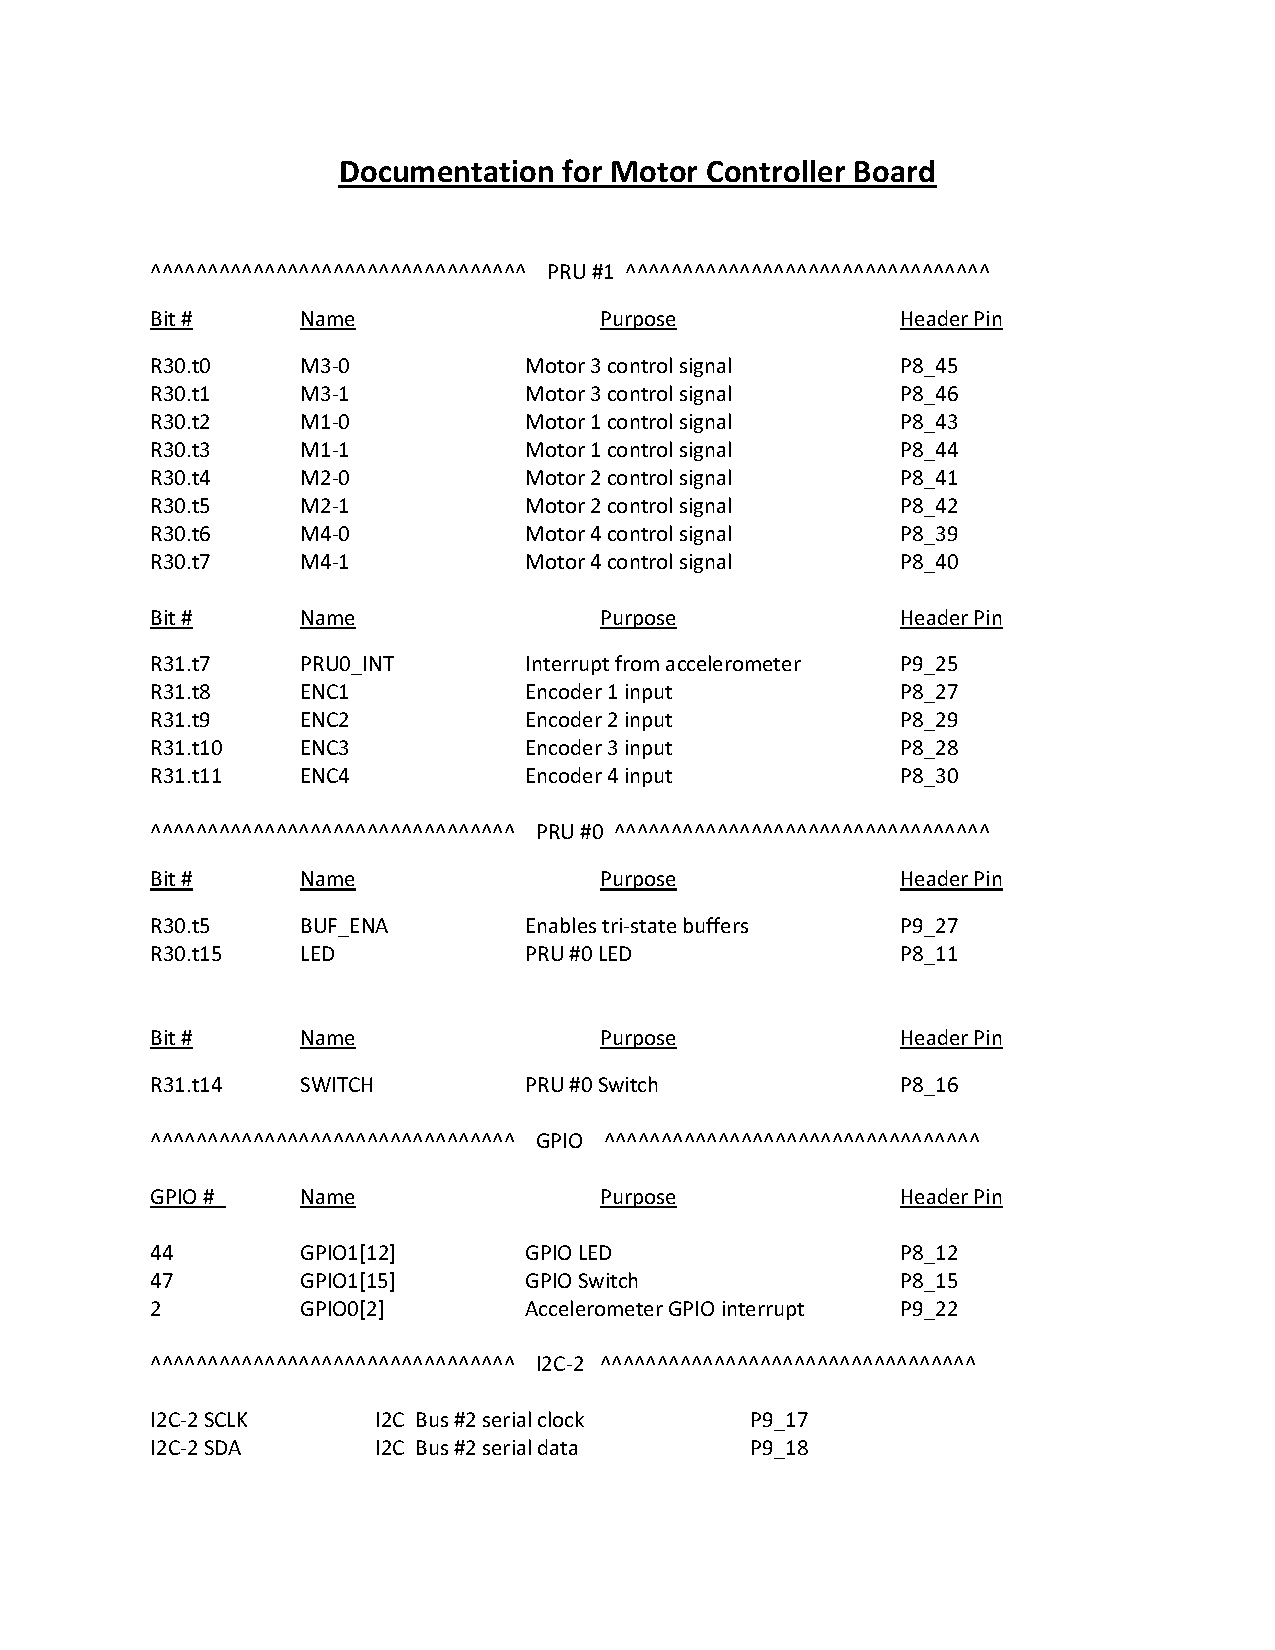
\includegraphics[scale=0.67,keepaspectratio=true]{./images/pins.pdf}
\end{figure}
\end{document}
